% Template f�r Diplomarbeit I
% ---------------------------
% angefertigt von Daniel Wilhelm (http://www.danielspage.de), 2010
% f�r ComTec (http://www.comtec.eecs.uni-kassel.de)


% Grundeinstellungen (Seitenformat, Sprache, etc.)
% Dokumentart, Seitenformat
\documentclass[pdftex, a4paper, twoside, open=right, parskip, numbers=noenddot, listof=totoc, bibliography=totocnumbered]{scrreprt}

% Seitenabst�nde
\usepackage[bindingoffset=1cm, left=2.5cm, right=2.5cm, top=2.5cm, bottom=2.5cm]{geometry}

% Code for creating empty pages
% No headers on empty pages before new chapter
\makeatletter
\def\cleardoublepage{\clearpage\if@twoside \ifodd\c@page\else
    \hbox{}
    \thispagestyle{plain}
    \newpage
    \if@twocolumn\hbox{}\newpage\fi\fi\fi}
\makeatother \clearpage{\pagestyle{plain}\cleardoublepage}

% Kopfzeilen
\usepackage{fancyhdr}
\pagestyle{fancy}
\renewcommand{\chaptermark}[1]{\markboth{\thechapter\ #1}{}}
\fancyhead[LO,RE]{\leftmark}
\fancyhead[RO,LE]{\thepage}
\cfoot{}
\fancypagestyle{plain}{}

% Eingabe von �, �, �, � erlauben
\usepackage[ansinew]{inputenc}
\usepackage[T1]{fontenc}

% Deutsche Trennungen, Anf�hrungsstriche und mehr:
\usepackage[ngerman]{babel}
\usepackage[babel, german=quotes]{csquotes}


% Farben einbinden
\usepackage{color}
\usepackage{colortbl}

% Farben
\definecolor{tableBlue}{RGB}{79, 129, 189} % Tabellen
\definecolor{lightyellow}{rgb}{1, 1, 0.8}  % Quellcode


% Tabellen
\usepackage{tabularx}
\usepackage{multirow}


% Bilder einbinden
\usepackage{graphicx, wrapfig}

% Fix zur Bildereinbindung
\renewcommand{\textfraction}{0}


% Hyperlinks
\usepackage[hyphens]{url}
\usepackage{hyperref}
\hypersetup{colorlinks, citecolor=black, linkcolor=black, urlcolor=black}


% Quellcode einbinden
\usepackage{listings}
\renewcommand{\lstlistlistingname}{Quellcodeverzeichnis}
\lstset{aboveskip=\bigskipamount, backgroundcolor=\color{lightyellow}, basicstyle=\ttfamily\small, breaklines, breakautoindent, captionpos=b, columns=flexible, extendedchars, float=hbp, frame=single, keywordstyle=\bfseries, language=C, numbers=left, numberstyle=\tiny, showspaces=false, showstringspaces=false, showtabs=false, stringstyle=, tabsize=2}


% Abk�rzungsverzeichnis
\usepackage[printonlyused]{acronym}

% Stiel des Literaturverzeichnisses.
\bibliographystyle{apalike}



% Dokument starten
\begin{document}
  % kleine r�mische Seitennummerierung
  \pagenumbering{roman}

  % Titelseite
  \begin{titlepage}
  % Schriftart ohne Serifen
  \sffamily

  % Logos und Schriftz�ge
  \begin{tabularx}{\textwidth}{@{}l@{}>{\raggedleft\arraybackslash}X@{}r@{}}
    \multirow{2}{*}{
\includegraphics[width=6.8cm]{title/Uni-Logo_4C}} &
    \raisebox{-1mm}{\small{Fachbereich Informatik}} \\
    & \raisebox{-3mm}{\small{Fachgebiet Bildverarbeitung}} &
  \end{tabularx}


  % Abstand
  \vspace{2.5cm}


  \begin{center}
    % Titel und Untertitel
    \huge\textsc{Lokalisation mobiler Roboter mit Odometrie und Bildverarbeitung in einer Theaterinstallation}

    % Abstand
    \vspace{3cm}

    % "Diplomarbeit 1"
    \renewcommand{\baselinestretch}{1.3}
    \Large\textsc{M A S T E R A R B E I T}


  \end{center}


  % Abstand
  \vspace{0.2cm}


  \renewcommand{\baselinestretch}{2}
  \large

  \begin{tabularx}{\textwidth}{XllX}
    eingereicht am \hspace{1cm} & 23.09.2013 & \\
     \\
    bei                         & Prof. Dr.-Ing. Udo Frese & \\
                                & Universit�t Bremen & \\
     \\
    von                         & Josef F. Hiller & \\
                                & Matr. Nr: 2055491 & \\
                                & Osterstr 79 & \\
                                & 28199 Bremen &
  \end{tabularx}

  \normalsize

  % Schriftart mit Serifen
  \rmfamily
\end{titlepage}


  % Texteinstellungen
  \renewcommand{\baselinestretch}{1.3}
  \large

  % Zusammenfassung
  \chapter*{Zusammenfassung}

% Inhaltsverzeichnis und Kopfzeile
\addcontentsline{toc}{chapter}{Zusammenfassung}
\markboth{Zusammenfassung}{Zusammenfassung}

  \vspace{0.5cm}

  \textbf{Schlagw�rter:} abc, def, xyz


  % Erkl�rung
  \chapter*{Erkl�rung}

% Inhaltsverzeichnis und Kopfzeile
\addcontentsline{toc}{chapter}{Erkl�rung}
\markboth{Erkl�rung}{Erkl�rung}

  Ich versichere, dass ich die vorliegende Arbeit selbstst�ndig angefertigt und mich fremder Hilfe nicht bedient habe. Alle Stellen, die w�rtlich oder sinngem�� ver�ffentlichtem oder unver�ffentlichtem Schrifttum entnommen sind, habe  ich als solche kenntlich gemacht.

  \vspace{1cm}

  Bremen, 23.09.2013

  \begin{flushright}
    \underline{\hspace{7cm}} \\
    Josef F. Hiller
  \end{flushright}


  % Zitat
  %% Inhaltsverzeichnis und Kopfzeile
\addcontentsline{toc}{chapter}{Zitat}
\markboth{Zitat}{Zitat}

% Abstand
\vspace*{15cm}

% Zitat
\begin{quote}
  Der Kaffee muss hei� wie die H�lle, schwarz der Teufel, rein wie ein Engel und s�� wie die Liebe sein.
\end{quote}

% Quelle
\begin{flushright}
  \textbf{Charles-Maurice de Talleyrand-P�rigord}
\end{flushright}


  % Verzeichnisse
  \addtocontents{toc}{\protect\vspace{0.2cm}}
  \tableofcontents
  \listoffigures
  \listoftables
  \lstlistoflistings

  % arabische Seitennummerierung
  \newpage
  \mbox{}  
  \newpage
  \pagenumbering{arabic}
  \addtocontents{toc}{\protect\vspace{1.0cm}}

  % Kapitel
  \chapter{Einleitung}

  Sed turpis erat (Abbildung \ref{Sprungmarke1}), tincidunt eu sollicitudin eu, tempus quis lectus. Nullam orci leo, tempus vitae dictum eu, bibendum at ante. In placerat, mi eu consequat suscipit, turpis arcu dictum tellus, nec scelerisque turpis eros a enim. Mauris quis leo lacus. Vestibulum condimentum porttitor malesuada. Pellentesque nec dictum nisl. Donec eleifend libero sit amet urna dignissim in faucibus lorem ultricies. Vestibulum interdum egestas metus vel porta. In vehicula leo at nibh dignissim malesuada. Etiam non nunc ligula. Vivamus vitae nibh dolor, eget faucibus tortor. Suspendisse ac quam enim. 

  \begin{figure}[htbp]
    \centering
    
\includegraphics[width=0.5\linewidth]{chapter1/RTEmagicC_fame_unscharf_03}
    \caption{Bildbeschreibung}
    \label{Sprungmarke1}
  \end{figure}

  Curabitur vitae velit nisl, vel sagittis arcu. Nullam sit amet ligula ut nibh ornare tempor. Pellentesque sollicitudin convallis dolor, eget pulvinar augue tempus sit amet. Aenean lacinia condimentum commodo. Pellentesque vestibulum mauris in orci sodales vitae tristique nulla tincidunt. Aenean tincidunt interdum est, a aliquet quam sollicitudin vel. Donec et lacus lorem. Nunc odio est, volutpat non rhoncus eu, dictum ut turpis. Fusce posuere rhoncus ipsum, nec pharetra nunc posuere bibendum. Morbi eu venenatis tortor.


  \section{Konzepte}

    Phasellus consectetur metus a sapien condimentum sodales. Sed ultrices sem turpis, in cursus turpis. Phasellus eleifend volutpat enim, ut varius tellus scelerisque et. Nulla facilisi. Integer congue gravida leo sit amet vulputate. Nam eu lacus nulla, eget sagittis arcu. Curabitur faucibus felis nulla, ut luctus justo. Lorem ipsum dolor sit amet, consectetur adipiscing elit. Curabitur mattis orci porta eros mattis sed ullamcorper erat volutpat. Nullam eu eros ut urna cursus posuere eu non neque. Nam suscipit mattis eros quis consectetur. Aliquam nec mi at metus iaculis fringilla ac euismod erat. Morbi id diam ac neque accumsan consequat. Nam laoreet facilisis placerat. Etiam interdum tincidunt dignissim. Nam facilisis vulputate elit, id dignissim dolor rhoncus nec. Vivamus pharetra laoreet dui tempus tincidunt.


  \section{Ziel und Aufgabenstellung der Arbeit}

  \begin{wrapfigure}{r}{5cm}
    \centering
    
\includegraphics{chapter1/Logo_ComTec}
    \caption[Von Text umflossenes Bild]{Wrapfigure}
    \label{fig:Wrap}
  \end{wrapfigure}

    Curabitur molestie egestas congue. Suspendisse erat urna, euismod at vulputate sit amet, scelerisque in arcu. Nam in est ac neque tristique mollis sit amet ac eros. Mauris felis ipsum, tincidunt at aliquam vel, faucibus vitae velit. Proin suscipit viverra vulputate. Nullam dignissim porttitor diam quis dictum. Cum sociis natoque penatibus et magnis dis parturient montes, nascetur ridiculus mus. Cras nulla urna, consectetur vitae laoreet ac, hendrerit in odio. Cras pellentesque luctus luctus. Donec ante nibh, dignissim ac semper sit amet, dictum eget libero. Donec elementum urna nec nisl feugiat et feugiat odio malesuada. Pellentesque pellentesque, leo in pharetra congue, leo augue bibendum leo, adipiscing aliquam sapien tellus eget odio. Cras et quam sed nibh iaculis convallis vitae nec est.


  \section{L�sungsweg der Aufgabenstellung}

    Cras pharetra rhoncus lacinia. Donec suscipit mattis arcu, sed mollis leo elementum vitae. Nam hendrerit, metus vitae ullamcorper pulvinar, neque velit aliquet massa, nec rhoncus neque erat at est. Proin ac lectus sit amet massa aliquam auctor. Phasellus non purus ac ante volutpat lacinia. Suspendisse ullamcorper libero nec libero auctor vulputate pretium arcu fermentum. Etiam vitae eros vitae justo viverra tempor. Quisque mauris mauris, dignissim non cursus tincidunt, ullamcorper sit amet nisi. Etiam tempor tellus et odio posuere ullamcorper. Class aptent taciti sociosqu ad litora torquent per conubia nostra, per inceptos himenaeos. Aliquam id nisi a augue commodo hendrerit. Maecenas arcu arcu, interdum pretium pulvinar vel, aliquam sed nisl. Nam sodales nulla nec massa mattis cursus. Sed vel fermentum nisi. Aliquam tristique sagittis sem, non pharetra ante auctor et. Phasellus vestibulum velit sed ipsum ullamcorper sit amet faucibus felis adipiscing. Nullam nec metus sit amet felis sodales blandit sed a neque. Ut sed erat a neque aliquet semper. Vestibulum id massa ut nulla posuere blandit id ut diam.


  \section{Gliederung}

    Nunc vitae tortor posuere ante viverra sollicitudin. Phasellus vestibulum est quis libero tincidunt lobortis. Suspendisse potenti. Pellentesque sit amet nisi id turpis pellentesque sodales. Morbi dui lectus, posuere ut adipiscing non, consectetur vitae odio. Fusce ut urna metus, quis tristique urna. Nunc faucibus euismod dui egestas sagittis. Aenean eu mauris ut libero adipiscing fermentum. Sed vitae lectus turpis, quis porta nisi. Vestibulum vel tortor sit amet urna bibendum scelerisque vel eu est. Suspendisse potenti. Nam odio tellus, consequat vitae faucibus quis, tincidunt at mi. Aliquam ut turpis lorem. Sed ut urna sit amet risus scelerisque consectetur. Donec porta aliquam est, quis iaculis nisl sagittis consequat. Curabitur in orci nisi. Nullam ipsum elit, convallis eget interdum at, imperdiet ut ligula.

  \chapter{Grundlagen}
\label{chap:grundlagen}

\section{Lokalisation}
\label{sec:lokalisation}
Die Lokalisation ist eines der Grundprobleme das beim Einsatz von mobilen Robotern auftritt.
In \cite[Seite 193]{Thrun2006} wird die sie in drei Teilprobleme zerlegt:
\begin{description}
\item[Position Tracking] bezeichnet den Vorgang, bei dem mit bekannter Ausgangsposition diese mit Hilfe von Sensordaten bei Bewegungen verfolgt werden kann. Dabei spielt das Dynamikmodell des Roboters sowie darin modellierte Unsicherheiten eine wichtige Rolle. Denn bewegt sich der Roboter von einer bekannten Position aus, wird mit dem Dynamikmodell seine neue Position gesch�tzt. Die Unsicherheiten des Modells erzeugen dabei eine Wahrscheinlichkeitsverteilung um diese neue Position, in der sich die wahre Position befinden sollte. Ohne Messungen von weiteren Sensoren die R�ckschl�sse auf die Umgebung erlauben, w�rde die Positionssch�tzung mit der Zeit immer ungenauer. Mit Hilfe eines Messmodells l�sst sich beurteilen, ob eine Messung an einer Bestimmten Position wahrscheinlich erscheint, oder nicht. Dadurch l�sst sich die Wahrscheinlichkeitsverteilung der Position nach einer Bewegung durch eine Messung wieder eingrenzen. Auf den Bereich, in dem der Messwert des Sensors am Wahrscheinlichsten ist.
\item[Global Localization] ist das finden der Anfangsposition des Roboters unter allen M�glichen Posen die im Szenario vorkommen k�nnen. Im Vergleich zum \textit{Position Tracking}, bei dem es gen�gte die Unsicherheit um die gesch�tzte neue Pose zu ber�cksichtigen, umfasst hier der Raum m�glicher Posen ein erheblich gr��eres Volumen. Ein Ansatz w�re alle m�glichen Posen mit der selben Wahrscheinlichkeit anzunehmen, und mit den ersten Messungen und dem Messmodell diese einzugrenzen. Auf Bereiche in denen diese Messungen mit hoher Wahrscheinlichkeit auftritt. 
\item[Kidnapped Robot Problem] ist eine versch�rfte Variante des \textit{Global Localization} Problems. Dabei geht man davon aus, das sich der Roboter spontan an einem anderen Ort aufh�lt als vom Roboter angenommen. Nun m�sste die Lokalisation des Roboters wieder im gesamten m�glichen Raum erfolgen. Nur das der Roboter diesen Zustand nicht feststellen kann. 
\end{description}

\subsection{�bersicht g�ngiger Verfahren}
\label{subsec:uebersichtVerfahren}
Die meisten L�sungsans�tze verwenden im Grunde eine Variante des Bayes-Filters wie z.B. in \cite[Seite 26]{Thrun2006} beschrieben. Abh�ngig vom Einsatzumfeld und der verwendeten Hardware gibt es aber noch Andere Verfahren.

In \cite{seco2009survey} zum Beispiel werden, neben dem Bayes-Filter, drei weitere genannt: \textit{Geometry-Based Methods}, \textit{Minimization of the cost function} und \textit{Fingerprint Methods} die sich in Geb�uden unter Nutzung von Elektromagnetischen Signale verwenden lassen. Je nach Sensorausstattung werden verschiedene Karten der Umgebung verwendet. Auf die sich der Roboter durch Auswertung von Sensormessungen lokalisieren muss. Dabei gibt es Karten die vorher angefertigt wurden, und dem Roboter bereits zur Verf�gung stehen. Und es gibt Karten die der Roboter selbstst�ndig w�hrend der Lokalisation erstellen muss. Letzteres wird als \ac{SLAM} Problem bezeichnet zu dem es bereits viele Ver�ffentlichungen gibt (u.a.) \cite[Seite 309]{Thrun2006}, \cite{Thrun:2002:PFR:2073876.2073937}, \cite[Seite 229]{Hertzberg2012}

Der in Kapitel \ref{chap:einleitung} erw�hnte Partikel Filter ist eine Variante des Bayes-Filters. Er ist auch auch als \ac{MCL} bekannt. Weitere Verfahren sind zum Beispiel: \textsc{Kalman Filter} (EKF, UKF), \textsc{Grid-Based-Filter} oder \textsc{Histogram Filter (continous Space)}, \textsc{discrete Bayes Filter (discrete Space)}

\cite{Thrun:2002:PFR:2073876.2073937} 

\subsection{Der Partikel Filter}
\label{subsec:partikelfilter}

\section{Bildverarbeitung}
\label{sec:bildverarbeitung}

\subsection{Projektion aus dem Raum auf die Bildebene}
\label{subsec:projektion}


  \chapter{Versuche in der Simulation}
\label{chap:versuche}
Die Versuche in diesem Kapitel sollen helfen das entwickelte Verfahren zu bewerten. Zun�chst wird eine Versuch beschrieben, in dem das Messmodell des Partikel-Filters untersucht wurde. Danach wird anhand von verschiedenen Fahrkurven das Verhalten bei unterschiedlichen Bildaufnahmefrequenzen betrachtet, sowie der Einfluss von Personen auf der B�hne beurteilt.

Wenn nicht anders angegeben, werden folgende Einstellungen f�r Simulation und Lokalisation verwendet:

\begin{tabular}{cc}
	\begin{minipage}{0.45\textwidth}
		\begin{description}
		\item[test1] hallo
		\item[test3] moin
		\end{description}
	\end{minipage} & 
	\begin{minipage}{0.45\textwidth}
		\begin{description}
		\item[test2] hallo2
		\item[test4] moin4
		\end{description}
	\end{minipage}
\end{tabular} 
\section{Versuche zur Genauigkeit des Messmodells}
\label{sec:VersucheModell}
In einer ersten Versuchsreihe, soll die Genauigkeit des im Partikelfilter verwendeten Messmodells untersucht werden. Daf�r soll zu einem gegebenen Bild m�glichst der gesamte Zustandsraum mit dem in Kapitel \ref{subsec:messmodell} beschriebenen Verfahren bewertet werden. Die Anzahl der Punkte im Zustandsraum, die einen hohen Score erhalten, l�sst darauf schlie�en wie genau die Zuordnung zwischen Bild und Pose funktioniert. Im ersten Durchlauf soll zun�chst grob der gesamte Raum abgesucht werden. Er soll einen �berblick geben, wo Antworten liegen, die dann in weiteren Durchl�ufen genauer abgetastet werden k�nnen.

\begin{figure}[p]
    \centering
    \vspace{-40pt}
    % GNUPLOT: LaTeX picture with Postscript
\begingroup
  \makeatletter
  \providecommand\color[2][]{%
    \GenericError{(gnuplot) \space\space\space\@spaces}{%
      Package color not loaded in conjunction with
      terminal option `colourtext'%
    }{See the gnuplot documentation for explanation.%
    }{Either use 'blacktext' in gnuplot or load the package
      color.sty in LaTeX.}%
    \renewcommand\color[2][]{}%
  }%
  \providecommand\includegraphics[2][]{%
    \GenericError{(gnuplot) \space\space\space\@spaces}{%
      Package graphicx or graphics not loaded%
    }{See the gnuplot documentation for explanation.%
    }{The gnuplot epslatex terminal needs graphicx.sty or graphics.sty.}%
    \renewcommand\includegraphics[2][]{}%
  }%
  \providecommand\rotatebox[2]{#2}%
  \@ifundefined{ifGPcolor}{%
    \newif\ifGPcolor
    \GPcolortrue
  }{}%
  \@ifundefined{ifGPblacktext}{%
    \newif\ifGPblacktext
    \GPblacktexttrue
  }{}%
  % define a \g@addto@macro without @ in the name:
  \let\gplgaddtomacro\g@addto@macro
  % define empty templates for all commands taking text:
  \gdef\gplbacktext{}%
  \gdef\gplfronttext{}%
  \makeatother
  \ifGPblacktext
    % no textcolor at all
    \def\colorrgb#1{}%
    \def\colorgray#1{}%
  \else
    % gray or color?
    \ifGPcolor
      \def\colorrgb#1{\color[rgb]{#1}}%
      \def\colorgray#1{\color[gray]{#1}}%
      \expandafter\def\csname LTw\endcsname{\color{white}}%
      \expandafter\def\csname LTb\endcsname{\color{black}}%
      \expandafter\def\csname LTa\endcsname{\color{black}}%
      \expandafter\def\csname LT0\endcsname{\color[rgb]{1,0,0}}%
      \expandafter\def\csname LT1\endcsname{\color[rgb]{0,1,0}}%
      \expandafter\def\csname LT2\endcsname{\color[rgb]{0,0,1}}%
      \expandafter\def\csname LT3\endcsname{\color[rgb]{1,0,1}}%
      \expandafter\def\csname LT4\endcsname{\color[rgb]{0,1,1}}%
      \expandafter\def\csname LT5\endcsname{\color[rgb]{1,1,0}}%
      \expandafter\def\csname LT6\endcsname{\color[rgb]{0,0,0}}%
      \expandafter\def\csname LT7\endcsname{\color[rgb]{1,0.3,0}}%
      \expandafter\def\csname LT8\endcsname{\color[rgb]{0.5,0.5,0.5}}%
    \else
      % gray
      \def\colorrgb#1{\color{black}}%
      \def\colorgray#1{\color[gray]{#1}}%
      \expandafter\def\csname LTw\endcsname{\color{white}}%
      \expandafter\def\csname LTb\endcsname{\color{black}}%
      \expandafter\def\csname LTa\endcsname{\color{black}}%
      \expandafter\def\csname LT0\endcsname{\color{black}}%
      \expandafter\def\csname LT1\endcsname{\color{black}}%
      \expandafter\def\csname LT2\endcsname{\color{black}}%
      \expandafter\def\csname LT3\endcsname{\color{black}}%
      \expandafter\def\csname LT4\endcsname{\color{black}}%
      \expandafter\def\csname LT5\endcsname{\color{black}}%
      \expandafter\def\csname LT6\endcsname{\color{black}}%
      \expandafter\def\csname LT7\endcsname{\color{black}}%
      \expandafter\def\csname LT8\endcsname{\color{black}}%
    \fi
  \fi
  \setlength{\unitlength}{0.0500bp}%
  \begin{picture}(8640.00,7200.00)%
    \gplgaddtomacro\gplbacktext{%
    }%
    \gplgaddtomacro\gplfronttext{%
      \csname LTb\endcsname%
      \put(5811,5663){\makebox(0,0)[r]{\strut{}     0.8}}%
      \csname LTb\endcsname%
      \put(5811,5443){\makebox(0,0)[r]{\strut{}     0.6}}%
      \csname LTb\endcsname%
      \put(5811,5223){\makebox(0,0)[r]{\strut{}     0.4}}%
      \csname LTb\endcsname%
      \put(5811,5003){\makebox(0,0)[r]{\strut{}     0.2}}%
      \csname LTb\endcsname%
      \put(2155,1078){\makebox(0,0){\strut{}-6}}%
      \csname LTb\endcsname%
      \put(4320,1078){\makebox(0,0){\strut{} 0}}%
      \csname LTb\endcsname%
      \put(6485,1078){\makebox(0,0){\strut{} 6}}%
      \put(4320,748){\makebox(0,0){\strut{}XAchse in Metern}}%
      \csname LTb\endcsname%
      \put(1802,1545){\makebox(0,0)[r]{\strut{}-6}}%
      \csname LTb\endcsname%
      \put(1802,3710){\makebox(0,0)[r]{\strut{} 0}}%
      \csname LTb\endcsname%
      \put(1802,5875){\makebox(0,0)[r]{\strut{} 6}}%
      \put(1472,3710){\rotatebox{-270}{\makebox(0,0){\strut{}YAchse in Metern}}}%
    }%
    \gplbacktext
    \put(0,0){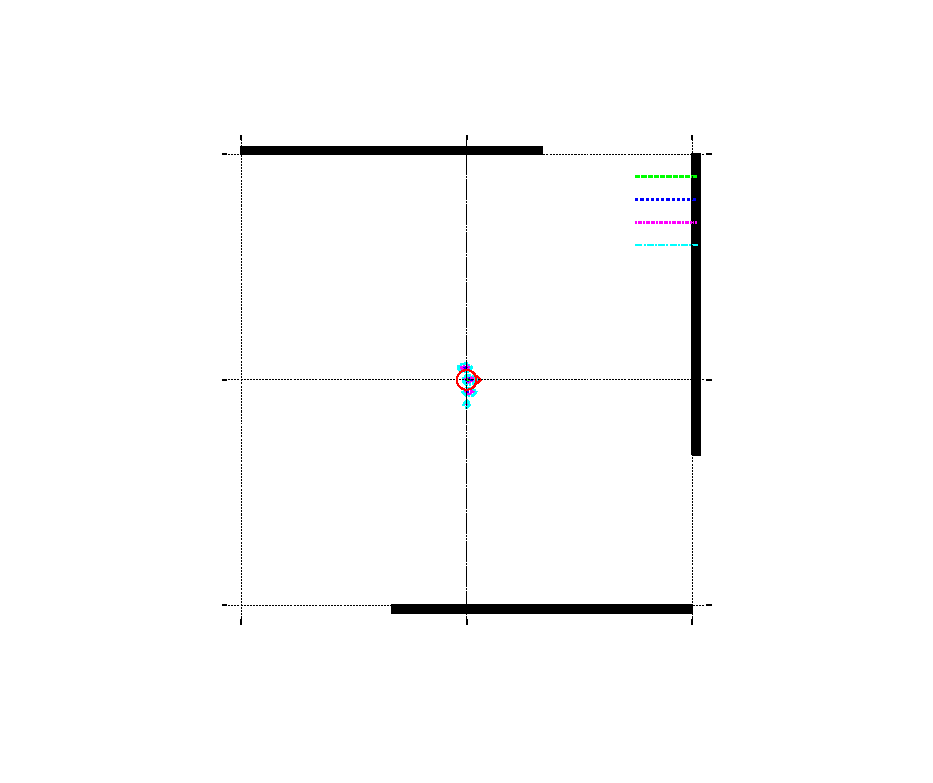
\includegraphics{chapter3/messmodell/full_6x6_5cm_005Deg}}%
    \gplfronttext
  \end{picture}%
\endgroup

    \vspace{-20pt}
    % GNUPLOT: LaTeX picture with Postscript
\begingroup
  \makeatletter
  \providecommand\color[2][]{%
    \GenericError{(gnuplot) \space\space\space\@spaces}{%
      Package color not loaded in conjunction with
      terminal option `colourtext'%
    }{See the gnuplot documentation for explanation.%
    }{Either use 'blacktext' in gnuplot or load the package
      color.sty in LaTeX.}%
    \renewcommand\color[2][]{}%
  }%
  \providecommand\includegraphics[2][]{%
    \GenericError{(gnuplot) \space\space\space\@spaces}{%
      Package graphicx or graphics not loaded%
    }{See the gnuplot documentation for explanation.%
    }{The gnuplot epslatex terminal needs graphicx.sty or graphics.sty.}%
    \renewcommand\includegraphics[2][]{}%
  }%
  \providecommand\rotatebox[2]{#2}%
  \@ifundefined{ifGPcolor}{%
    \newif\ifGPcolor
    \GPcolortrue
  }{}%
  \@ifundefined{ifGPblacktext}{%
    \newif\ifGPblacktext
    \GPblacktexttrue
  }{}%
  % define a \g@addto@macro without @ in the name:
  \let\gplgaddtomacro\g@addto@macro
  % define empty templates for all commands taking text:
  \gdef\gplbacktext{}%
  \gdef\gplfronttext{}%
  \makeatother
  \ifGPblacktext
    % no textcolor at all
    \def\colorrgb#1{}%
    \def\colorgray#1{}%
  \else
    % gray or color?
    \ifGPcolor
      \def\colorrgb#1{\color[rgb]{#1}}%
      \def\colorgray#1{\color[gray]{#1}}%
      \expandafter\def\csname LTw\endcsname{\color{white}}%
      \expandafter\def\csname LTb\endcsname{\color{black}}%
      \expandafter\def\csname LTa\endcsname{\color{black}}%
      \expandafter\def\csname LT0\endcsname{\color[rgb]{1,0,0}}%
      \expandafter\def\csname LT1\endcsname{\color[rgb]{0,1,0}}%
      \expandafter\def\csname LT2\endcsname{\color[rgb]{0,0,1}}%
      \expandafter\def\csname LT3\endcsname{\color[rgb]{1,0,1}}%
      \expandafter\def\csname LT4\endcsname{\color[rgb]{0,1,1}}%
      \expandafter\def\csname LT5\endcsname{\color[rgb]{1,1,0}}%
      \expandafter\def\csname LT6\endcsname{\color[rgb]{0,0,0}}%
      \expandafter\def\csname LT7\endcsname{\color[rgb]{1,0.3,0}}%
      \expandafter\def\csname LT8\endcsname{\color[rgb]{0.5,0.5,0.5}}%
    \else
      % gray
      \def\colorrgb#1{\color{black}}%
      \def\colorgray#1{\color[gray]{#1}}%
      \expandafter\def\csname LTw\endcsname{\color{white}}%
      \expandafter\def\csname LTb\endcsname{\color{black}}%
      \expandafter\def\csname LTa\endcsname{\color{black}}%
      \expandafter\def\csname LT0\endcsname{\color{black}}%
      \expandafter\def\csname LT1\endcsname{\color{black}}%
      \expandafter\def\csname LT2\endcsname{\color{black}}%
      \expandafter\def\csname LT3\endcsname{\color{black}}%
      \expandafter\def\csname LT4\endcsname{\color{black}}%
      \expandafter\def\csname LT5\endcsname{\color{black}}%
      \expandafter\def\csname LT6\endcsname{\color{black}}%
      \expandafter\def\csname LT7\endcsname{\color{black}}%
      \expandafter\def\csname LT8\endcsname{\color{black}}%
    \fi
  \fi
  \setlength{\unitlength}{0.0500bp}%
  \begin{picture}(8640.00,7200.00)%
    \gplgaddtomacro\gplbacktext{%
    }%
    \gplgaddtomacro\gplfronttext{%
      \csname LTb\endcsname%
      \put(5811,5663){\makebox(0,0)[r]{\strut{}     0.8}}%
      \csname LTb\endcsname%
      \put(5811,5443){\makebox(0,0)[r]{\strut{}     0.6}}%
      \csname LTb\endcsname%
      \put(5811,5223){\makebox(0,0)[r]{\strut{}     0.4}}%
      \csname LTb\endcsname%
      \put(5811,5003){\makebox(0,0)[r]{\strut{}     0.2}}%
      \csname LTb\endcsname%
      \put(1974,1078){\makebox(0,0){\strut{}-0.5}}%
      \csname LTb\endcsname%
      \put(2443,1078){\makebox(0,0){\strut{}-0.4}}%
      \csname LTb\endcsname%
      \put(2913,1078){\makebox(0,0){\strut{}-0.3}}%
      \csname LTb\endcsname%
      \put(3382,1078){\makebox(0,0){\strut{}-0.2}}%
      \csname LTb\endcsname%
      \put(3851,1078){\makebox(0,0){\strut{}-0.1}}%
      \csname LTb\endcsname%
      \put(4320,1078){\makebox(0,0){\strut{} 0}}%
      \csname LTb\endcsname%
      \put(4789,1078){\makebox(0,0){\strut{} 0.1}}%
      \csname LTb\endcsname%
      \put(5258,1078){\makebox(0,0){\strut{} 0.2}}%
      \csname LTb\endcsname%
      \put(5727,1078){\makebox(0,0){\strut{} 0.3}}%
      \csname LTb\endcsname%
      \put(6197,1078){\makebox(0,0){\strut{} 0.4}}%
      \csname LTb\endcsname%
      \put(6666,1078){\makebox(0,0){\strut{} 0.5}}%
      \put(4320,748){\makebox(0,0){\strut{}XAchse in Metern}}%
      \csname LTb\endcsname%
      \put(1802,1364){\makebox(0,0)[r]{\strut{}-0.5}}%
      \csname LTb\endcsname%
      \put(1802,1833){\makebox(0,0)[r]{\strut{}-0.4}}%
      \csname LTb\endcsname%
      \put(1802,2303){\makebox(0,0)[r]{\strut{}-0.3}}%
      \csname LTb\endcsname%
      \put(1802,2772){\makebox(0,0)[r]{\strut{}-0.2}}%
      \csname LTb\endcsname%
      \put(1802,3241){\makebox(0,0)[r]{\strut{}-0.1}}%
      \csname LTb\endcsname%
      \put(1802,3710){\makebox(0,0)[r]{\strut{} 0}}%
      \csname LTb\endcsname%
      \put(1802,4179){\makebox(0,0)[r]{\strut{} 0.1}}%
      \csname LTb\endcsname%
      \put(1802,4648){\makebox(0,0)[r]{\strut{} 0.2}}%
      \csname LTb\endcsname%
      \put(1802,5117){\makebox(0,0)[r]{\strut{} 0.3}}%
      \csname LTb\endcsname%
      \put(1802,5587){\makebox(0,0)[r]{\strut{} 0.4}}%
      \csname LTb\endcsname%
      \put(1802,6056){\makebox(0,0)[r]{\strut{} 0.5}}%
      \put(1208,3710){\rotatebox{-270}{\makebox(0,0){\strut{}YAchse in Metern}}}%
    }%
    \gplbacktext
    \put(0,0){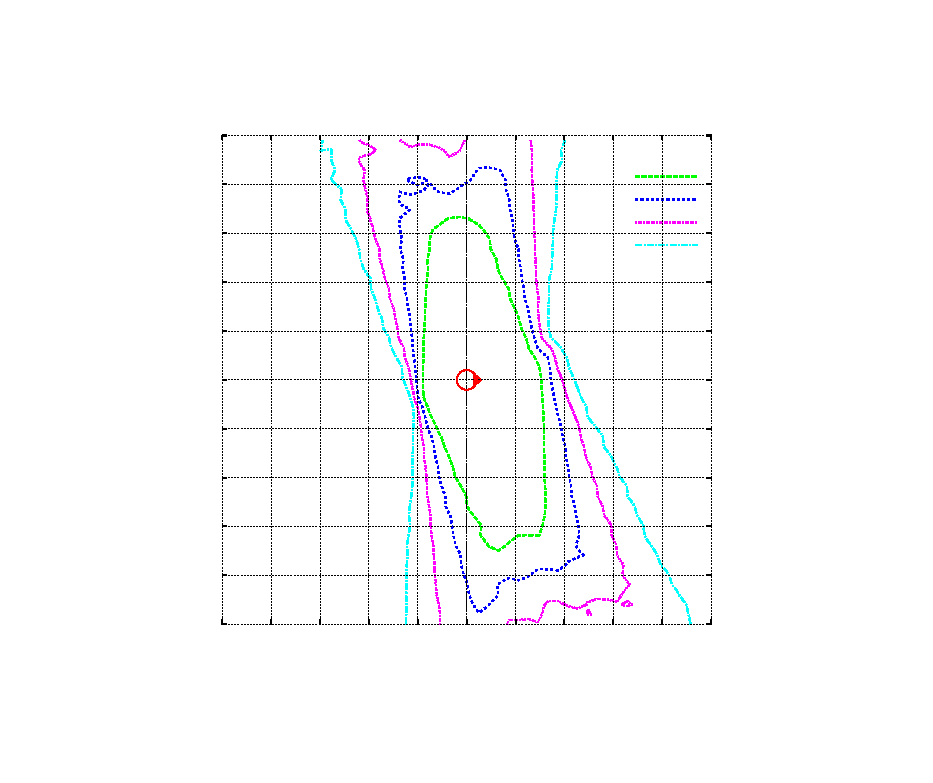
\includegraphics{chapter3/messmodell/position_variance_on_picture}}%
    \gplfronttext
  \end{picture}%
\endgroup

    \caption[Antwort des Messmodells im Zustandsraum auf ein gegebenes Bild]{Antwort des Messmodells zu einem Bild an der rot markierten Position oben: 5\,$cm$ Raster 3� Schritte unten: 1\,$cm$ Raster 0.3� Schritte}
    \label{fig:messmodellPos}
\end{figure}

F�r die Versuchsreihe wird der Zustandsraum zun�chst grob in 5\,$cm$ Rasterschritten durchsucht. Dabei wird die Orientierung in 0,05 Rad (2,86�) Schritte aufgeteilt. In drei Schleifen wird so der Zustandsraum durchlaufen. Als Messung wurde ein am Ursprung (x = 0, y = 0, psi = 0) aufgenommenes Bild verwendet. F�r die Darstellung in Abbildung \ref{fig:messmodellPos} oben, wurden H�henlinien der Messantwort eingezeichnet. Dabei wurde jeweils nur die st�rkste Antwort an einer Position �ber alle Winkel gew�hlt. Bei einem Zweiten Durchlauf wurde die Positionsrasterung auf 1\,cm Schritte und die Winkelschritte auf 0,005 Rad (0.28�) verkleinert. Zu sehen ist dies auf Abbildung \ref{fig:messmodellPos} unten. Um den Einfluss des Winkels darzustellen wurde in Abbildung \ref{fig:messmodellAngle} die Antwort entlang einer Linie mit $x=0.0$ geplottet. 

In Abbildung \ref{fig:messmodellPos} oben ist der Zustandsraum der Position dargestellt. Die Orientierung konnte in dieser Abbildung nicht gezeigt werden. Die Lichtw�nde wurden als schwarze Balken kenntlich gemacht. Der rote Kreis zeigt die Pose des Roboters als das Bild aufgenommen wurde. Eine Antwort des Messmodells ist nur um die diese Position zu sehen, in dem Rest des Zustandsraumes (B�hne) gab es keine signifikante Antwort. Auf dem Bild darunter sieht man einen Vergr��erten Ausschnitt um die Roboterposition. Hier f�llt auf, dass die H�ufung leicht schr�g liegt. Der Grund daf�r ist vermutlich, dass die Lichtwand auf der das Muster abgebildet ist, nicht zentral vor dem Roboter steht, sondern in Y-Richtung verschoben ist. Die H�ufung der Antworten streut vor allem entlang der Y-Achse, dies entspricht einer seitlichen Verschiebung des Roboters entlang dieser Achse bei gleichzeitiger Drehung. Dabei sind innerhalb von $\pm 30$\,$cm$ immer noch Scores gr��er als 0,8 m�glich. Entlang der X-Achse ist eine Streuung zwischen $+15$ und $-10$\,cm zu erkennen. Durch die H�henlinien ist zu erkennen, dass entlang der x-Achse der Score eine gro�e Steigung hat. Dies f�hrt zu einer relativ scharfen Kante in dieser Richtung. Auf der y-Achse dagegen, ist die Steigung schw�cher, dadurch bildet sich keine scharfe Kante. 
Aus Abbildung \ref{fig:messmodellAngle} l�sst sich entnehmen, dass bei einer Verschiebung entlang der Y-Achse eine Drehung des Roboters n�tig ist, um eine Pose zu erhalten die einen guten Score erh�lt.
\begin{figure}[h]
    \centering
    % GNUPLOT: LaTeX picture with Postscript
\begingroup
  \makeatletter
  \providecommand\color[2][]{%
    \GenericError{(gnuplot) \space\space\space\@spaces}{%
      Package color not loaded in conjunction with
      terminal option `colourtext'%
    }{See the gnuplot documentation for explanation.%
    }{Either use 'blacktext' in gnuplot or load the package
      color.sty in LaTeX.}%
    \renewcommand\color[2][]{}%
  }%
  \providecommand\includegraphics[2][]{%
    \GenericError{(gnuplot) \space\space\space\@spaces}{%
      Package graphicx or graphics not loaded%
    }{See the gnuplot documentation for explanation.%
    }{The gnuplot epslatex terminal needs graphicx.sty or graphics.sty.}%
    \renewcommand\includegraphics[2][]{}%
  }%
  \providecommand\rotatebox[2]{#2}%
  \@ifundefined{ifGPcolor}{%
    \newif\ifGPcolor
    \GPcolortrue
  }{}%
  \@ifundefined{ifGPblacktext}{%
    \newif\ifGPblacktext
    \GPblacktexttrue
  }{}%
  % define a \g@addto@macro without @ in the name:
  \let\gplgaddtomacro\g@addto@macro
  % define empty templates for all commands taking text:
  \gdef\gplbacktext{}%
  \gdef\gplfronttext{}%
  \makeatother
  \ifGPblacktext
    % no textcolor at all
    \def\colorrgb#1{}%
    \def\colorgray#1{}%
  \else
    % gray or color?
    \ifGPcolor
      \def\colorrgb#1{\color[rgb]{#1}}%
      \def\colorgray#1{\color[gray]{#1}}%
      \expandafter\def\csname LTw\endcsname{\color{white}}%
      \expandafter\def\csname LTb\endcsname{\color{black}}%
      \expandafter\def\csname LTa\endcsname{\color{black}}%
      \expandafter\def\csname LT0\endcsname{\color[rgb]{1,0,0}}%
      \expandafter\def\csname LT1\endcsname{\color[rgb]{0,1,0}}%
      \expandafter\def\csname LT2\endcsname{\color[rgb]{0,0,1}}%
      \expandafter\def\csname LT3\endcsname{\color[rgb]{1,0,1}}%
      \expandafter\def\csname LT4\endcsname{\color[rgb]{0,1,1}}%
      \expandafter\def\csname LT5\endcsname{\color[rgb]{1,1,0}}%
      \expandafter\def\csname LT6\endcsname{\color[rgb]{0,0,0}}%
      \expandafter\def\csname LT7\endcsname{\color[rgb]{1,0.3,0}}%
      \expandafter\def\csname LT8\endcsname{\color[rgb]{0.5,0.5,0.5}}%
    \else
      % gray
      \def\colorrgb#1{\color{black}}%
      \def\colorgray#1{\color[gray]{#1}}%
      \expandafter\def\csname LTw\endcsname{\color{white}}%
      \expandafter\def\csname LTb\endcsname{\color{black}}%
      \expandafter\def\csname LTa\endcsname{\color{black}}%
      \expandafter\def\csname LT0\endcsname{\color{black}}%
      \expandafter\def\csname LT1\endcsname{\color{black}}%
      \expandafter\def\csname LT2\endcsname{\color{black}}%
      \expandafter\def\csname LT3\endcsname{\color{black}}%
      \expandafter\def\csname LT4\endcsname{\color{black}}%
      \expandafter\def\csname LT5\endcsname{\color{black}}%
      \expandafter\def\csname LT6\endcsname{\color{black}}%
      \expandafter\def\csname LT7\endcsname{\color{black}}%
      \expandafter\def\csname LT8\endcsname{\color{black}}%
    \fi
  \fi
  \setlength{\unitlength}{0.0500bp}%
  \begin{picture}(8640.00,7200.00)%
    \gplgaddtomacro\gplbacktext{%
    }%
    \gplgaddtomacro\gplfronttext{%
      \csname LTb\endcsname%
      \put(5811,5663){\makebox(0,0)[r]{\strut{}     0.8}}%
      \csname LTb\endcsname%
      \put(5811,5443){\makebox(0,0)[r]{\strut{}     0.6}}%
      \csname LTb\endcsname%
      \put(5811,5223){\makebox(0,0)[r]{\strut{}     0.4}}%
      \csname LTb\endcsname%
      \put(5811,5003){\makebox(0,0)[r]{\strut{}     0.2}}%
      \csname LTb\endcsname%
      \put(1974,1078){\makebox(0,0){\strut{}-6}}%
      \csname LTb\endcsname%
      \put(2365,1078){\makebox(0,0){\strut{}-5}}%
      \csname LTb\endcsname%
      \put(2756,1078){\makebox(0,0){\strut{}-4}}%
      \csname LTb\endcsname%
      \put(3147,1078){\makebox(0,0){\strut{}-3}}%
      \csname LTb\endcsname%
      \put(3538,1078){\makebox(0,0){\strut{}-2}}%
      \csname LTb\endcsname%
      \put(3929,1078){\makebox(0,0){\strut{}-1}}%
      \csname LTb\endcsname%
      \put(4320,1078){\makebox(0,0){\strut{} 0}}%
      \csname LTb\endcsname%
      \put(4711,1078){\makebox(0,0){\strut{} 1}}%
      \csname LTb\endcsname%
      \put(5102,1078){\makebox(0,0){\strut{} 2}}%
      \csname LTb\endcsname%
      \put(5493,1078){\makebox(0,0){\strut{} 3}}%
      \csname LTb\endcsname%
      \put(5884,1078){\makebox(0,0){\strut{} 4}}%
      \csname LTb\endcsname%
      \put(6275,1078){\makebox(0,0){\strut{} 5}}%
      \csname LTb\endcsname%
      \put(6666,1078){\makebox(0,0){\strut{} 6}}%
      \put(4320,748){\makebox(0,0){\strut{}XAchse Winkel in Grad}}%
      \csname LTb\endcsname%
      \put(1802,1364){\makebox(0,0)[r]{\strut{}-0.5}}%
      \csname LTb\endcsname%
      \put(1802,1833){\makebox(0,0)[r]{\strut{}-0.4}}%
      \csname LTb\endcsname%
      \put(1802,2303){\makebox(0,0)[r]{\strut{}-0.3}}%
      \csname LTb\endcsname%
      \put(1802,2772){\makebox(0,0)[r]{\strut{}-0.2}}%
      \csname LTb\endcsname%
      \put(1802,3241){\makebox(0,0)[r]{\strut{}-0.1}}%
      \csname LTb\endcsname%
      \put(1802,3710){\makebox(0,0)[r]{\strut{} 0}}%
      \csname LTb\endcsname%
      \put(1802,4179){\makebox(0,0)[r]{\strut{} 0.1}}%
      \csname LTb\endcsname%
      \put(1802,4648){\makebox(0,0)[r]{\strut{} 0.2}}%
      \csname LTb\endcsname%
      \put(1802,5117){\makebox(0,0)[r]{\strut{} 0.3}}%
      \csname LTb\endcsname%
      \put(1802,5587){\makebox(0,0)[r]{\strut{} 0.4}}%
      \csname LTb\endcsname%
      \put(1802,6056){\makebox(0,0)[r]{\strut{} 0.5}}%
      \put(1208,3710){\rotatebox{-270}{\makebox(0,0){\strut{}YAchse in Metern}}}%
    }%
    \gplbacktext
    \put(0,0){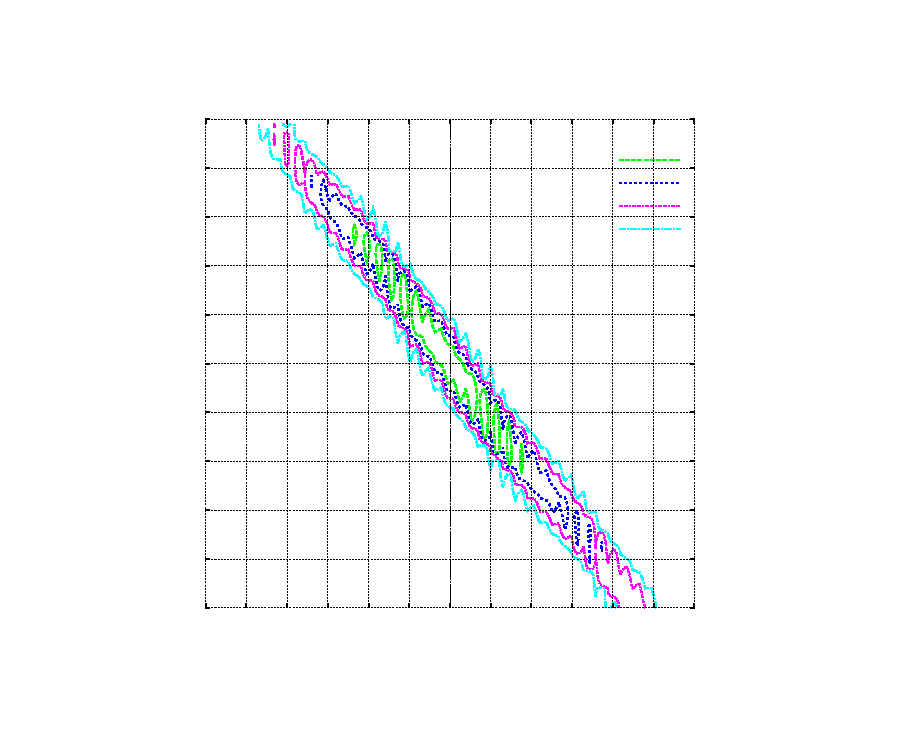
\includegraphics{chapter3/messmodell/pTOyANDangle_1cm_0005Deg_xIS0}}%
    \gplfronttext
  \end{picture}%
\endgroup

    \caption{Antwort des Messmodells bei x=0.0}
    \label{fig:messmodellAngle}
\end{figure}

\section{Verwendete Fahrkurven}
\label{sec:Fahrkurven}
Es sind vier verschiedene Fahrkurven f�r die folgenden zwei Versuche verwendet worden. An dieser Stelle soll kurz auf Besonderheiten hingewiesen werden, die f�r diese Kurven beobachtet wurden. F�r alle Kurven gilt, dass sie in der Mitte der B�hne beginnen, und die Lokalisation mit der Startposition initialisiert ist. Die Versuche beziehen sich somit nur auf das Pose Tracking der Lokalisation. Auf den Abbildungen \ref{fig:FahrLoopsAntiTop} und \ref{fig:FahrSchlangenTop} sind die Lichtw�nde zur Orientierung als schwarze Rechtecke in die Diagramme eingezeichnet worden. Bei den Simulationen f�r diese Fahrkurven wurden alle 1500\,ms Bilder der Kamera ausgewertet. Die blauen Ellipsen sind die $3\sigma$ Vertrauensbereiche um die gesch�tzte Position des Roboters. Sie wurden f�r einzelne Stichproben eingezeichnet.

\begin{description}
\item[Loop Anticlockwise] Ist eine Fahrt entlang der �u�eren Kanten der B�hne, dabei f�hrt der Roboter gegen den Uhrzeigersinn.
Die Lichtw�nde stehen nicht auf der Ganzen L�nge der B�hne, sondern immer versetzt. Dies f�hrt bei dieser Fahrtrichtung dazu, dass die Lichtw�nde seltener im Bild sichtbar sind. Es m�ssten weniger Bit-Musterpunkte im Bild zu sehen sein, als bei der Fahrt im Uhrzeigersinn. Aber genug um einen Score zu bilden. Zu sehen auf Abbildung~\ref{fig:FahrLoopsAntiTop} oben auf Seite~\pageref{fig:FahrLoopsAntiTop}. Es ist zu erkennen, dass auch entlang der offenen Seite die Unsicherheit gro� bleibt, obwohl auf eine Lichtw�nde zu gefahren wird. Dies liegt vermutlich an der Versetzt aufgestellten Wand. Der Roboter f�hrt hier auf ein offenes St�ck zu und die Mess-Updates reichen nicht um die Position genauer eingrenzen zu k�nnen.
\item[Loop Clockwise] F�hrt die gleiche Strecke von \textbf{Loop~Anticlockwise} entlang, nur im Uhrzeigersinn. Die Kamera des Roboters ist die meiste Zeit auf mindestens eine Lichtwand gerichtet. Nur wenn er auf die offene Seite zu f�hrt erh�lt er kein auswertbares Messupdate. Zu sehen auf Abbildung~\ref{fig:FahrLoopsAntiTop} unten auf Seite~\pageref{fig:FahrLoopsAntiTop}. Die Unsicherheit der Position nimmt auf dem St�ck zur offenen Seite hin deutlich zu, sobald wieder eine Lichtwand von der Kamera erfasst wird, nimmt sie wieder ab.
\end{description}
\begin{figure}[p]
    \centering
    \vspace{-30pt}
    % GNUPLOT: LaTeX picture with Postscript
\begingroup
  \makeatletter
  \providecommand\color[2][]{%
    \GenericError{(gnuplot) \space\space\space\@spaces}{%
      Package color not loaded in conjunction with
      terminal option `colourtext'%
    }{See the gnuplot documentation for explanation.%
    }{Either use 'blacktext' in gnuplot or load the package
      color.sty in LaTeX.}%
    \renewcommand\color[2][]{}%
  }%
  \providecommand\includegraphics[2][]{%
    \GenericError{(gnuplot) \space\space\space\@spaces}{%
      Package graphicx or graphics not loaded%
    }{See the gnuplot documentation for explanation.%
    }{The gnuplot epslatex terminal needs graphicx.sty or graphics.sty.}%
    \renewcommand\includegraphics[2][]{}%
  }%
  \providecommand\rotatebox[2]{#2}%
  \@ifundefined{ifGPcolor}{%
    \newif\ifGPcolor
    \GPcolortrue
  }{}%
  \@ifundefined{ifGPblacktext}{%
    \newif\ifGPblacktext
    \GPblacktexttrue
  }{}%
  % define a \g@addto@macro without @ in the name:
  \let\gplgaddtomacro\g@addto@macro
  % define empty templates for all commands taking text:
  \gdef\gplbacktext{}%
  \gdef\gplfronttext{}%
  \makeatother
  \ifGPblacktext
    % no textcolor at all
    \def\colorrgb#1{}%
    \def\colorgray#1{}%
  \else
    % gray or color?
    \ifGPcolor
      \def\colorrgb#1{\color[rgb]{#1}}%
      \def\colorgray#1{\color[gray]{#1}}%
      \expandafter\def\csname LTw\endcsname{\color{white}}%
      \expandafter\def\csname LTb\endcsname{\color{black}}%
      \expandafter\def\csname LTa\endcsname{\color{black}}%
      \expandafter\def\csname LT0\endcsname{\color[rgb]{1,0,0}}%
      \expandafter\def\csname LT1\endcsname{\color[rgb]{0,1,0}}%
      \expandafter\def\csname LT2\endcsname{\color[rgb]{0,0,1}}%
      \expandafter\def\csname LT3\endcsname{\color[rgb]{1,0,1}}%
      \expandafter\def\csname LT4\endcsname{\color[rgb]{0,1,1}}%
      \expandafter\def\csname LT5\endcsname{\color[rgb]{1,1,0}}%
      \expandafter\def\csname LT6\endcsname{\color[rgb]{0,0,0}}%
      \expandafter\def\csname LT7\endcsname{\color[rgb]{1,0.3,0}}%
      \expandafter\def\csname LT8\endcsname{\color[rgb]{0.5,0.5,0.5}}%
    \else
      % gray
      \def\colorrgb#1{\color{black}}%
      \def\colorgray#1{\color[gray]{#1}}%
      \expandafter\def\csname LTw\endcsname{\color{white}}%
      \expandafter\def\csname LTb\endcsname{\color{black}}%
      \expandafter\def\csname LTa\endcsname{\color{black}}%
      \expandafter\def\csname LT0\endcsname{\color{black}}%
      \expandafter\def\csname LT1\endcsname{\color{black}}%
      \expandafter\def\csname LT2\endcsname{\color{black}}%
      \expandafter\def\csname LT3\endcsname{\color{black}}%
      \expandafter\def\csname LT4\endcsname{\color{black}}%
      \expandafter\def\csname LT5\endcsname{\color{black}}%
      \expandafter\def\csname LT6\endcsname{\color{black}}%
      \expandafter\def\csname LT7\endcsname{\color{black}}%
      \expandafter\def\csname LT8\endcsname{\color{black}}%
    \fi
  \fi
  \setlength{\unitlength}{0.0500bp}%
  \begin{picture}(6480.00,7200.00)%
    \gplgaddtomacro\gplbacktext{%
      \csname LTb\endcsname%
      \put(682,2569){\makebox(0,0)[r]{\strut{}-6}}%
      \csname LTb\endcsname%
      \put(682,4149){\makebox(0,0)[r]{\strut{} 0}}%
      \csname LTb\endcsname%
      \put(682,5730){\makebox(0,0)[r]{\strut{} 6}}%
      \csname LTb\endcsname%
      \put(1868,1295){\makebox(0,0){\strut{}-6}}%
      \csname LTb\endcsname%
      \put(3448,1295){\makebox(0,0){\strut{} 0}}%
      \csname LTb\endcsname%
      \put(5029,1295){\makebox(0,0){\strut{} 6}}%
      \csname LTb\endcsname%
      \put(176,4149){\rotatebox{-270}{\makebox(0,0){\strut{}Y-Achse in Metern}}}%
      \put(3448,965){\makebox(0,0){\strut{}X-Achse in Metern}}%
    }%
    \gplgaddtomacro\gplfronttext{%
      \csname LTb\endcsname%
      \put(2593,393){\makebox(0,0)[r]{\strut{}$3\sigma$}}%
      \csname LTb\endcsname%
      \put(2593,173){\makebox(0,0)[r]{\strut{}Trajektorie}}%
      \csname LTb\endcsname%
      \put(5560,393){\makebox(0,0)[r]{\strut{}Filter Sch�tzung}}%
      \csname LTb\endcsname%
      \put(5560,173){\makebox(0,0)[r]{\strut{}Update}}%
    }%
    \gplbacktext
    \put(0,0){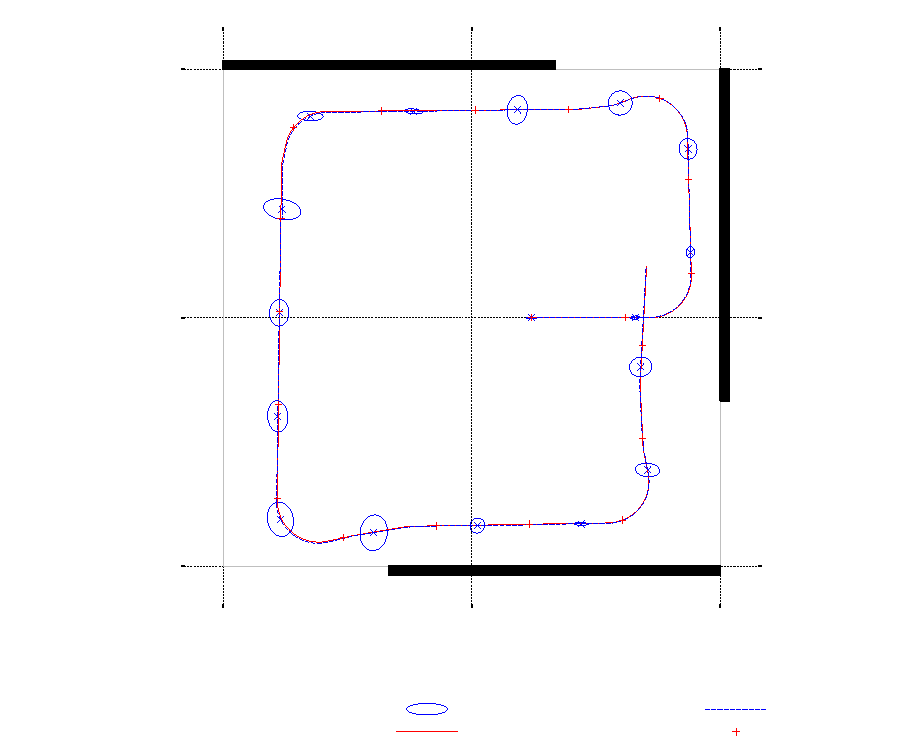
\includegraphics{chapter3/fahrkurven/Loop_Anticlockwise_1500}}%
    \gplfronttext
  \end{picture}%
\endgroup

    \vspace{-10pt}
    % GNUPLOT: LaTeX picture with Postscript
\begingroup
  \makeatletter
  \providecommand\color[2][]{%
    \GenericError{(gnuplot) \space\space\space\@spaces}{%
      Package color not loaded in conjunction with
      terminal option `colourtext'%
    }{See the gnuplot documentation for explanation.%
    }{Either use 'blacktext' in gnuplot or load the package
      color.sty in LaTeX.}%
    \renewcommand\color[2][]{}%
  }%
  \providecommand\includegraphics[2][]{%
    \GenericError{(gnuplot) \space\space\space\@spaces}{%
      Package graphicx or graphics not loaded%
    }{See the gnuplot documentation for explanation.%
    }{The gnuplot epslatex terminal needs graphicx.sty or graphics.sty.}%
    \renewcommand\includegraphics[2][]{}%
  }%
  \providecommand\rotatebox[2]{#2}%
  \@ifundefined{ifGPcolor}{%
    \newif\ifGPcolor
    \GPcolortrue
  }{}%
  \@ifundefined{ifGPblacktext}{%
    \newif\ifGPblacktext
    \GPblacktexttrue
  }{}%
  % define a \g@addto@macro without @ in the name:
  \let\gplgaddtomacro\g@addto@macro
  % define empty templates for all commands taking text:
  \gdef\gplbacktext{}%
  \gdef\gplfronttext{}%
  \makeatother
  \ifGPblacktext
    % no textcolor at all
    \def\colorrgb#1{}%
    \def\colorgray#1{}%
  \else
    % gray or color?
    \ifGPcolor
      \def\colorrgb#1{\color[rgb]{#1}}%
      \def\colorgray#1{\color[gray]{#1}}%
      \expandafter\def\csname LTw\endcsname{\color{white}}%
      \expandafter\def\csname LTb\endcsname{\color{black}}%
      \expandafter\def\csname LTa\endcsname{\color{black}}%
      \expandafter\def\csname LT0\endcsname{\color[rgb]{1,0,0}}%
      \expandafter\def\csname LT1\endcsname{\color[rgb]{0,1,0}}%
      \expandafter\def\csname LT2\endcsname{\color[rgb]{0,0,1}}%
      \expandafter\def\csname LT3\endcsname{\color[rgb]{1,0,1}}%
      \expandafter\def\csname LT4\endcsname{\color[rgb]{0,1,1}}%
      \expandafter\def\csname LT5\endcsname{\color[rgb]{1,1,0}}%
      \expandafter\def\csname LT6\endcsname{\color[rgb]{0,0,0}}%
      \expandafter\def\csname LT7\endcsname{\color[rgb]{1,0.3,0}}%
      \expandafter\def\csname LT8\endcsname{\color[rgb]{0.5,0.5,0.5}}%
    \else
      % gray
      \def\colorrgb#1{\color{black}}%
      \def\colorgray#1{\color[gray]{#1}}%
      \expandafter\def\csname LTw\endcsname{\color{white}}%
      \expandafter\def\csname LTb\endcsname{\color{black}}%
      \expandafter\def\csname LTa\endcsname{\color{black}}%
      \expandafter\def\csname LT0\endcsname{\color{black}}%
      \expandafter\def\csname LT1\endcsname{\color{black}}%
      \expandafter\def\csname LT2\endcsname{\color{black}}%
      \expandafter\def\csname LT3\endcsname{\color{black}}%
      \expandafter\def\csname LT4\endcsname{\color{black}}%
      \expandafter\def\csname LT5\endcsname{\color{black}}%
      \expandafter\def\csname LT6\endcsname{\color{black}}%
      \expandafter\def\csname LT7\endcsname{\color{black}}%
      \expandafter\def\csname LT8\endcsname{\color{black}}%
    \fi
  \fi
  \setlength{\unitlength}{0.0500bp}%
  \begin{picture}(8640.00,7200.00)%
    \gplgaddtomacro\gplbacktext{%
      \csname LTb\endcsname%
      \put(1611,1762){\makebox(0,0)[r]{\strut{}-6}}%
      \csname LTb\endcsname%
      \put(1611,4150){\makebox(0,0)[r]{\strut{} 0}}%
      \csname LTb\endcsname%
      \put(1611,6537){\makebox(0,0)[r]{\strut{} 6}}%
      \csname LTb\endcsname%
      \put(2141,1144){\makebox(0,0){\strut{}-6}}%
      \csname LTb\endcsname%
      \put(4529,1144){\makebox(0,0){\strut{} 0}}%
      \csname LTb\endcsname%
      \put(6916,1144){\makebox(0,0){\strut{} 6}}%
      \csname LTb\endcsname%
      \put(1105,4149){\rotatebox{-270}{\makebox(0,0){\strut{}Y-Achse in Metern}}}%
      \put(4528,814){\makebox(0,0){\strut{}X-Achse in Metern}}%
    }%
    \gplgaddtomacro\gplfronttext{%
      \csname LTb\endcsname%
      \put(3673,393){\makebox(0,0)[r]{\strut{}$3\sigma$}}%
      \csname LTb\endcsname%
      \put(3673,173){\makebox(0,0)[r]{\strut{}Trajektorie}}%
      \csname LTb\endcsname%
      \put(6640,393){\makebox(0,0)[r]{\strut{}Filter Sch�tzung}}%
      \csname LTb\endcsname%
      \put(6640,173){\makebox(0,0)[r]{\strut{}Update}}%
    }%
    \gplbacktext
    \put(0,0){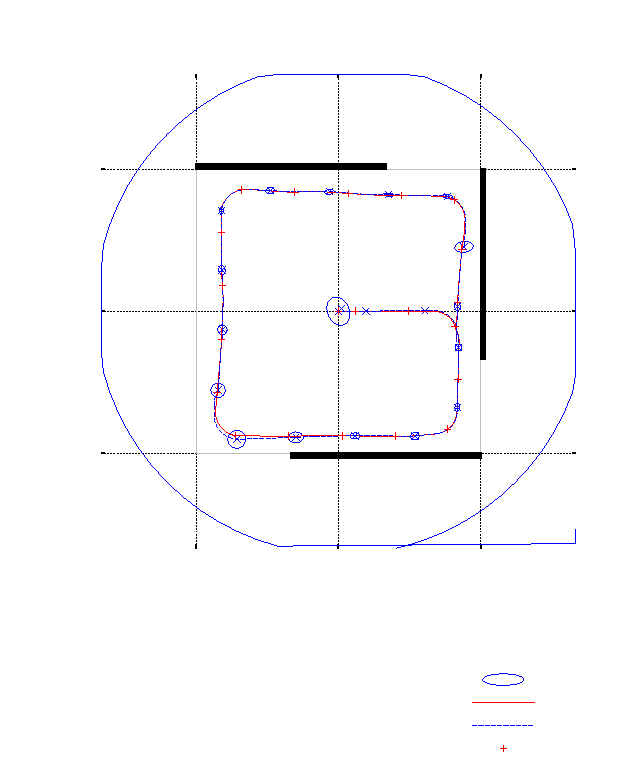
\includegraphics{chapter3/fahrkurven/Loop_Clockwise_1500}}%
    \gplfronttext
  \end{picture}%
\endgroup

    \caption{Fahrkurven oben Loop~Anticlockwise, und unten Loop~Clockwise}
    \label{fig:FahrLoopsAntiTop}
\end{figure}

\begin{description}
\item[Schlangenlinien] Bei dieser Fahrt f�hrt der Roboter mehrere male zwischen der Seite ohne Lichtwand und  der ihr gegen�ber liegenden Lichtwand hin und her. Dabei f�hrt er in Schlangenlinien die B�hne ab. In dieser Fahrkurve sind besonders viele scharfe Kurve enthalten. Des weiteren wird immer wieder auf die offene Seite zu gefahren, so dass es zeitweise keine auswertbaren Bilder gibt. Zu sehen auf Abbildung~\ref{fig:FahrSchlangenTop} oben auf Seite~\pageref{fig:FahrSchlangenTop}. Besonders stark wird die Unsicherheit wenn der Roboter oben links im Diagramm dicht an der Lichtwand entlang und auf die offene Seite zu f�hrt. Es ist au�erdem gut zu erkennen, wie die Unsicherheit gr��er wird, wenn der Roboter in negativer x-Richtung auf die offene Seite zu f�hrt und wieder kleiner wird, wenn er in positiver x-Richtung auf die Lichtwand zu f�hrt.
\item[Ellipse] Eine schr�ge Ellipse die um den Mittelpunkt liegt. Dabei f�hrt der Roboter etwa die H�lfte der Strecke auf zwei Lichtw�nde zu und die andere H�lfte auf die Ecke der B�hne in der  keine Lichtw�nde stehen. W�hrend er auf die offene Seite zu f�hrt, sieht er zeitweise keine Lichtwand um einen verwertbare Messung zu erhalten. Zu sehen auf Abbildung~\ref{fig:FahrSchlangenTop} unten auf Seite~\pageref{fig:FahrSchlangenTop}. Entsprechend verh�lt sich die Unsicherheit auf diesem Abschnitt. Sie wird gr��er, bis wieder eine Lichtwand in das Gesichtsfeld der Kamera kommt. Auf der Fahrt auf die Lichtw�nde zu bleibt die Unsicherheit klein.
\end{description}

\section{Versuche zur Bildaufnahmefrequenz}
\label{sec:versucheFrequenz}
Es soll untersucht werden in welchen Intervallen Bilder ben�tigt werden, wie stark der Einfluss der Fahrkurve darauf ist, und welche Faktoren die Bildaufnahmefrequenz beeinflussen k�nnen. Dazu werden die vier beschriebenen Fahrkurven eingesetzt. Sie werden in einem Simulationslauf dreimal abgefahren. Bei diesem Vorgang wird der Abstand zwischen der wahren und der vom Filter gesch�tzten Position des Roboters errechnet und �ber die Simulationsdauer ein Mittelwert $\hat{d}$ bestimmt.
\begin{equation}
\hat{d}=\frac{1}{n}\sum\limits_{i=0}^n \sqrt{(x_i-xtrue_i)^2+(y_i-ytrue_i)^2}
\end{equation}
Um zus�tzlich noch ein Ma� f�r die Genauigkeit der gesch�tzten Position zu haben, wird der Mittelwert der gro�en Achse der Unsicherheits-Ellipsen gebildet:
\begin{equation}
\hat{a}=\frac{1}{n}\sum\limits_{i=0}^n a_i
\end{equation} 
\vspace{10pt}

\begin{figure}[hp]
    \centering
    \vspace{-30pt}
    % GNUPLOT: LaTeX picture with Postscript
\begingroup
  \makeatletter
  \providecommand\color[2][]{%
    \GenericError{(gnuplot) \space\space\space\@spaces}{%
      Package color not loaded in conjunction with
      terminal option `colourtext'%
    }{See the gnuplot documentation for explanation.%
    }{Either use 'blacktext' in gnuplot or load the package
      color.sty in LaTeX.}%
    \renewcommand\color[2][]{}%
  }%
  \providecommand\includegraphics[2][]{%
    \GenericError{(gnuplot) \space\space\space\@spaces}{%
      Package graphicx or graphics not loaded%
    }{See the gnuplot documentation for explanation.%
    }{The gnuplot epslatex terminal needs graphicx.sty or graphics.sty.}%
    \renewcommand\includegraphics[2][]{}%
  }%
  \providecommand\rotatebox[2]{#2}%
  \@ifundefined{ifGPcolor}{%
    \newif\ifGPcolor
    \GPcolortrue
  }{}%
  \@ifundefined{ifGPblacktext}{%
    \newif\ifGPblacktext
    \GPblacktexttrue
  }{}%
  % define a \g@addto@macro without @ in the name:
  \let\gplgaddtomacro\g@addto@macro
  % define empty templates for all commands taking text:
  \gdef\gplbacktext{}%
  \gdef\gplfronttext{}%
  \makeatother
  \ifGPblacktext
    % no textcolor at all
    \def\colorrgb#1{}%
    \def\colorgray#1{}%
  \else
    % gray or color?
    \ifGPcolor
      \def\colorrgb#1{\color[rgb]{#1}}%
      \def\colorgray#1{\color[gray]{#1}}%
      \expandafter\def\csname LTw\endcsname{\color{white}}%
      \expandafter\def\csname LTb\endcsname{\color{black}}%
      \expandafter\def\csname LTa\endcsname{\color{black}}%
      \expandafter\def\csname LT0\endcsname{\color[rgb]{1,0,0}}%
      \expandafter\def\csname LT1\endcsname{\color[rgb]{0,1,0}}%
      \expandafter\def\csname LT2\endcsname{\color[rgb]{0,0,1}}%
      \expandafter\def\csname LT3\endcsname{\color[rgb]{1,0,1}}%
      \expandafter\def\csname LT4\endcsname{\color[rgb]{0,1,1}}%
      \expandafter\def\csname LT5\endcsname{\color[rgb]{1,1,0}}%
      \expandafter\def\csname LT6\endcsname{\color[rgb]{0,0,0}}%
      \expandafter\def\csname LT7\endcsname{\color[rgb]{1,0.3,0}}%
      \expandafter\def\csname LT8\endcsname{\color[rgb]{0.5,0.5,0.5}}%
    \else
      % gray
      \def\colorrgb#1{\color{black}}%
      \def\colorgray#1{\color[gray]{#1}}%
      \expandafter\def\csname LTw\endcsname{\color{white}}%
      \expandafter\def\csname LTb\endcsname{\color{black}}%
      \expandafter\def\csname LTa\endcsname{\color{black}}%
      \expandafter\def\csname LT0\endcsname{\color{black}}%
      \expandafter\def\csname LT1\endcsname{\color{black}}%
      \expandafter\def\csname LT2\endcsname{\color{black}}%
      \expandafter\def\csname LT3\endcsname{\color{black}}%
      \expandafter\def\csname LT4\endcsname{\color{black}}%
      \expandafter\def\csname LT5\endcsname{\color{black}}%
      \expandafter\def\csname LT6\endcsname{\color{black}}%
      \expandafter\def\csname LT7\endcsname{\color{black}}%
      \expandafter\def\csname LT8\endcsname{\color{black}}%
    \fi
  \fi
  \setlength{\unitlength}{0.0500bp}%
  \begin{picture}(8640.00,7200.00)%
    \gplgaddtomacro\gplbacktext{%
      \csname LTb\endcsname%
      \put(1611,1762){\makebox(0,0)[r]{\strut{}-6}}%
      \csname LTb\endcsname%
      \put(1611,4150){\makebox(0,0)[r]{\strut{} 0}}%
      \csname LTb\endcsname%
      \put(1611,6537){\makebox(0,0)[r]{\strut{} 6}}%
      \csname LTb\endcsname%
      \put(2141,1144){\makebox(0,0){\strut{}-6}}%
      \csname LTb\endcsname%
      \put(4529,1144){\makebox(0,0){\strut{} 0}}%
      \csname LTb\endcsname%
      \put(6916,1144){\makebox(0,0){\strut{} 6}}%
      \csname LTb\endcsname%
      \put(1105,4149){\rotatebox{-270}{\makebox(0,0){\strut{}Y-Achse in Metern}}}%
      \put(4528,814){\makebox(0,0){\strut{}X-Achse in Metern}}%
    }%
    \gplgaddtomacro\gplfronttext{%
      \csname LTb\endcsname%
      \put(3673,393){\makebox(0,0)[r]{\strut{}$3\sigma$}}%
      \csname LTb\endcsname%
      \put(3673,173){\makebox(0,0)[r]{\strut{}Trajektorie}}%
      \csname LTb\endcsname%
      \put(6640,393){\makebox(0,0)[r]{\strut{}Filter Sch�tzung}}%
      \csname LTb\endcsname%
      \put(6640,173){\makebox(0,0)[r]{\strut{}Update}}%
    }%
    \gplbacktext
    \put(0,0){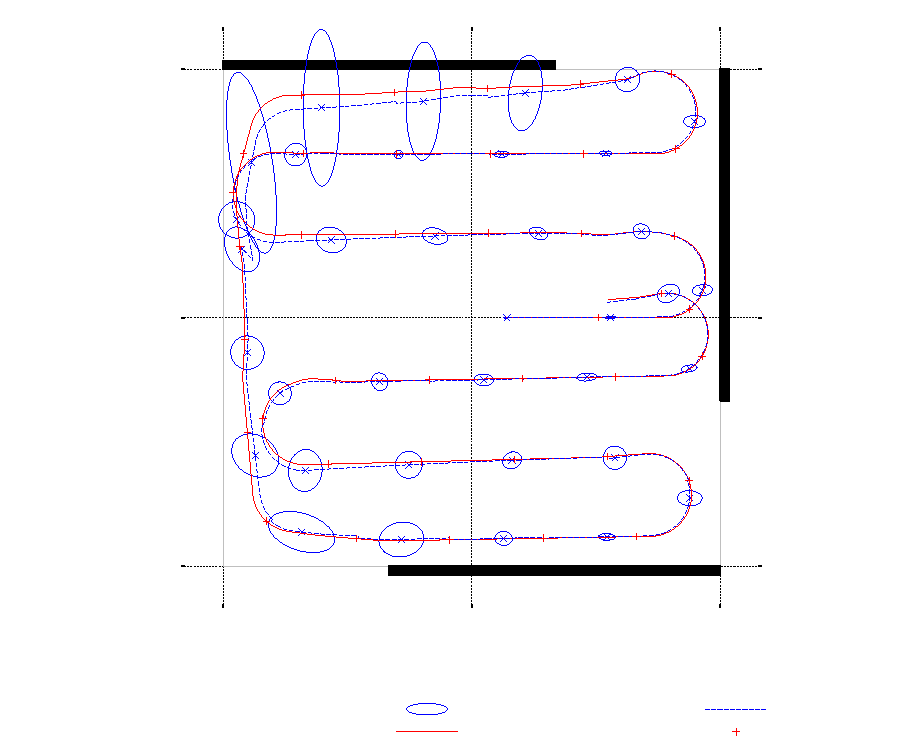
\includegraphics{chapter3/fahrkurven/serpentinen_1500}}%
    \gplfronttext
  \end{picture}%
\endgroup

    \vspace{-10pt}
    % GNUPLOT: LaTeX picture with Postscript
\begingroup
  \makeatletter
  \providecommand\color[2][]{%
    \GenericError{(gnuplot) \space\space\space\@spaces}{%
      Package color not loaded in conjunction with
      terminal option `colourtext'%
    }{See the gnuplot documentation for explanation.%
    }{Either use 'blacktext' in gnuplot or load the package
      color.sty in LaTeX.}%
    \renewcommand\color[2][]{}%
  }%
  \providecommand\includegraphics[2][]{%
    \GenericError{(gnuplot) \space\space\space\@spaces}{%
      Package graphicx or graphics not loaded%
    }{See the gnuplot documentation for explanation.%
    }{The gnuplot epslatex terminal needs graphicx.sty or graphics.sty.}%
    \renewcommand\includegraphics[2][]{}%
  }%
  \providecommand\rotatebox[2]{#2}%
  \@ifundefined{ifGPcolor}{%
    \newif\ifGPcolor
    \GPcolortrue
  }{}%
  \@ifundefined{ifGPblacktext}{%
    \newif\ifGPblacktext
    \GPblacktexttrue
  }{}%
  % define a \g@addto@macro without @ in the name:
  \let\gplgaddtomacro\g@addto@macro
  % define empty templates for all commands taking text:
  \gdef\gplbacktext{}%
  \gdef\gplfronttext{}%
  \makeatother
  \ifGPblacktext
    % no textcolor at all
    \def\colorrgb#1{}%
    \def\colorgray#1{}%
  \else
    % gray or color?
    \ifGPcolor
      \def\colorrgb#1{\color[rgb]{#1}}%
      \def\colorgray#1{\color[gray]{#1}}%
      \expandafter\def\csname LTw\endcsname{\color{white}}%
      \expandafter\def\csname LTb\endcsname{\color{black}}%
      \expandafter\def\csname LTa\endcsname{\color{black}}%
      \expandafter\def\csname LT0\endcsname{\color[rgb]{1,0,0}}%
      \expandafter\def\csname LT1\endcsname{\color[rgb]{0,1,0}}%
      \expandafter\def\csname LT2\endcsname{\color[rgb]{0,0,1}}%
      \expandafter\def\csname LT3\endcsname{\color[rgb]{1,0,1}}%
      \expandafter\def\csname LT4\endcsname{\color[rgb]{0,1,1}}%
      \expandafter\def\csname LT5\endcsname{\color[rgb]{1,1,0}}%
      \expandafter\def\csname LT6\endcsname{\color[rgb]{0,0,0}}%
      \expandafter\def\csname LT7\endcsname{\color[rgb]{1,0.3,0}}%
      \expandafter\def\csname LT8\endcsname{\color[rgb]{0.5,0.5,0.5}}%
    \else
      % gray
      \def\colorrgb#1{\color{black}}%
      \def\colorgray#1{\color[gray]{#1}}%
      \expandafter\def\csname LTw\endcsname{\color{white}}%
      \expandafter\def\csname LTb\endcsname{\color{black}}%
      \expandafter\def\csname LTa\endcsname{\color{black}}%
      \expandafter\def\csname LT0\endcsname{\color{black}}%
      \expandafter\def\csname LT1\endcsname{\color{black}}%
      \expandafter\def\csname LT2\endcsname{\color{black}}%
      \expandafter\def\csname LT3\endcsname{\color{black}}%
      \expandafter\def\csname LT4\endcsname{\color{black}}%
      \expandafter\def\csname LT5\endcsname{\color{black}}%
      \expandafter\def\csname LT6\endcsname{\color{black}}%
      \expandafter\def\csname LT7\endcsname{\color{black}}%
      \expandafter\def\csname LT8\endcsname{\color{black}}%
    \fi
  \fi
  \setlength{\unitlength}{0.0500bp}%
  \begin{picture}(5760.00,7200.00)%
    \gplgaddtomacro\gplbacktext{%
      \csname LTb\endcsname%
      \put(682,3005){\makebox(0,0)[r]{\strut{}-6}}%
      \csname LTb\endcsname%
      \put(682,4369){\makebox(0,0)[r]{\strut{} 0}}%
      \csname LTb\endcsname%
      \put(682,5734){\makebox(0,0)[r]{\strut{} 6}}%
      \csname LTb\endcsname%
      \put(1724,1875){\makebox(0,0){\strut{}-6}}%
      \csname LTb\endcsname%
      \put(3088,1875){\makebox(0,0){\strut{} 0}}%
      \csname LTb\endcsname%
      \put(4453,1875){\makebox(0,0){\strut{} 6}}%
      \csname LTb\endcsname%
      \put(176,4369){\rotatebox{-270}{\makebox(0,0){\strut{}Y-Achse in Metern}}}%
      \put(3088,1545){\makebox(0,0){\strut{}X-Achse in Metern}}%
    }%
    \gplgaddtomacro\gplfronttext{%
      \csname LTb\endcsname%
      \put(4245,833){\makebox(0,0)[r]{\strut{}$3\sigma$}}%
      \csname LTb\endcsname%
      \put(4245,613){\makebox(0,0)[r]{\strut{}Trajektorie des Roboters}}%
      \csname LTb\endcsname%
      \put(4245,393){\makebox(0,0)[r]{\strut{}Filter Sch�tzung}}%
      \csname LTb\endcsname%
      \put(4245,173){\makebox(0,0)[r]{\strut{}Update}}%
    }%
    \gplbacktext
    \put(0,0){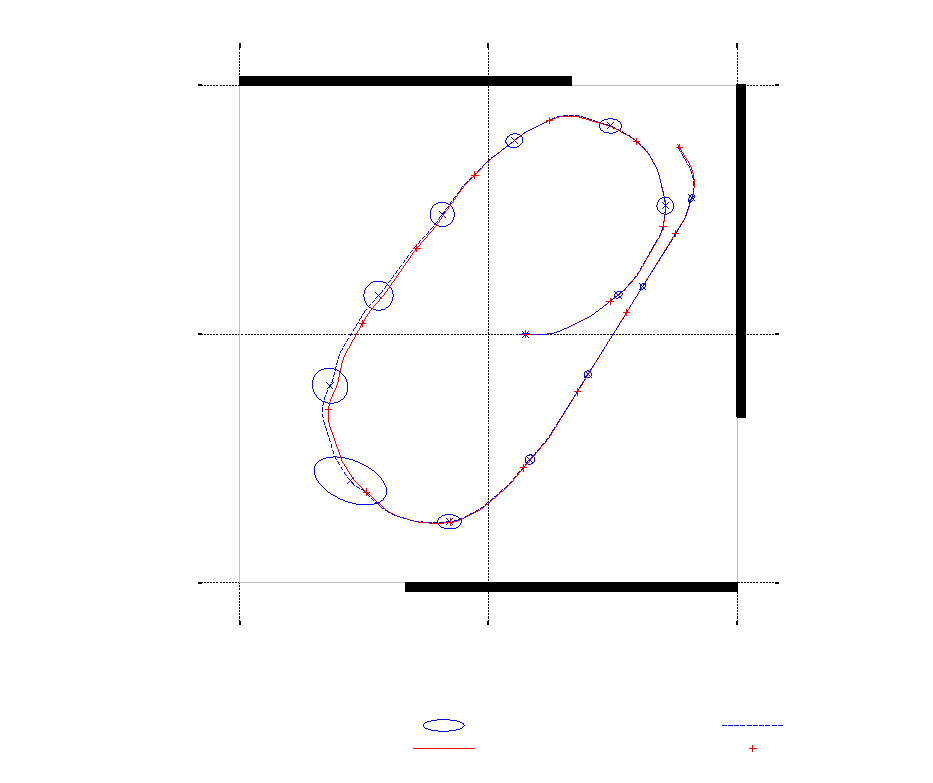
\includegraphics{chapter3/fahrkurven/Oval_1500}}%
    \gplfronttext
  \end{picture}%
\endgroup

    \caption{Fahrkurven oben Schlangenlinien, unten schr�ge Ellipse}
    \label{fig:FahrSchlangenTop}
\end{figure}

Jeder Simulationsdurchlauf arbeitet mit zuf�lligen systematischen Messabweichungen. Aus diesem Grund werden 15 Simulationsdurchl�ufe bei gleichen Einstellungen durchgef�hrt und �ber deren Ergebnisse gemittelt. Es wurden vier verschiedene Perioden f�r die Zeit zwischen zwei Bildern festgelegt: 500, 1000, 2000 und 4000\,$ms$. F�r jeden dieser Schritte wurde jede Fahrkurve damit 15 mal simuliert. 

\begin{figure}[h]
	\centering
	% GNUPLOT: LaTeX picture with Postscript
\begingroup
  \makeatletter
  \providecommand\color[2][]{%
    \GenericError{(gnuplot) \space\space\space\@spaces}{%
      Package color not loaded in conjunction with
      terminal option `colourtext'%
    }{See the gnuplot documentation for explanation.%
    }{Either use 'blacktext' in gnuplot or load the package
      color.sty in LaTeX.}%
    \renewcommand\color[2][]{}%
  }%
  \providecommand\includegraphics[2][]{%
    \GenericError{(gnuplot) \space\space\space\@spaces}{%
      Package graphicx or graphics not loaded%
    }{See the gnuplot documentation for explanation.%
    }{The gnuplot epslatex terminal needs graphicx.sty or graphics.sty.}%
    \renewcommand\includegraphics[2][]{}%
  }%
  \providecommand\rotatebox[2]{#2}%
  \@ifundefined{ifGPcolor}{%
    \newif\ifGPcolor
    \GPcolortrue
  }{}%
  \@ifundefined{ifGPblacktext}{%
    \newif\ifGPblacktext
    \GPblacktexttrue
  }{}%
  % define a \g@addto@macro without @ in the name:
  \let\gplgaddtomacro\g@addto@macro
  % define empty templates for all commands taking text:
  \gdef\gplbacktext{}%
  \gdef\gplfronttext{}%
  \makeatother
  \ifGPblacktext
    % no textcolor at all
    \def\colorrgb#1{}%
    \def\colorgray#1{}%
  \else
    % gray or color?
    \ifGPcolor
      \def\colorrgb#1{\color[rgb]{#1}}%
      \def\colorgray#1{\color[gray]{#1}}%
      \expandafter\def\csname LTw\endcsname{\color{white}}%
      \expandafter\def\csname LTb\endcsname{\color{black}}%
      \expandafter\def\csname LTa\endcsname{\color{black}}%
      \expandafter\def\csname LT0\endcsname{\color[rgb]{1,0,0}}%
      \expandafter\def\csname LT1\endcsname{\color[rgb]{0,1,0}}%
      \expandafter\def\csname LT2\endcsname{\color[rgb]{0,0,1}}%
      \expandafter\def\csname LT3\endcsname{\color[rgb]{1,0,1}}%
      \expandafter\def\csname LT4\endcsname{\color[rgb]{0,1,1}}%
      \expandafter\def\csname LT5\endcsname{\color[rgb]{1,1,0}}%
      \expandafter\def\csname LT6\endcsname{\color[rgb]{0,0,0}}%
      \expandafter\def\csname LT7\endcsname{\color[rgb]{1,0.3,0}}%
      \expandafter\def\csname LT8\endcsname{\color[rgb]{0.5,0.5,0.5}}%
    \else
      % gray
      \def\colorrgb#1{\color{black}}%
      \def\colorgray#1{\color[gray]{#1}}%
      \expandafter\def\csname LTw\endcsname{\color{white}}%
      \expandafter\def\csname LTb\endcsname{\color{black}}%
      \expandafter\def\csname LTa\endcsname{\color{black}}%
      \expandafter\def\csname LT0\endcsname{\color{black}}%
      \expandafter\def\csname LT1\endcsname{\color{black}}%
      \expandafter\def\csname LT2\endcsname{\color{black}}%
      \expandafter\def\csname LT3\endcsname{\color{black}}%
      \expandafter\def\csname LT4\endcsname{\color{black}}%
      \expandafter\def\csname LT5\endcsname{\color{black}}%
      \expandafter\def\csname LT6\endcsname{\color{black}}%
      \expandafter\def\csname LT7\endcsname{\color{black}}%
      \expandafter\def\csname LT8\endcsname{\color{black}}%
    \fi
  \fi
  \setlength{\unitlength}{0.0500bp}%
  \begin{picture}(8640.00,7200.00)%
    \gplgaddtomacro\gplbacktext{%
      \csname LTb\endcsname%
      \put(1078,704){\makebox(0,0)[r]{\strut{} 0}}%
      \put(1078,1743){\makebox(0,0)[r]{\strut{} 0.05}}%
      \put(1078,2781){\makebox(0,0)[r]{\strut{} 0.1}}%
      \put(1078,3820){\makebox(0,0)[r]{\strut{} 0.15}}%
      \put(1078,4858){\makebox(0,0)[r]{\strut{} 0.2}}%
      \put(1078,5897){\makebox(0,0)[r]{\strut{} 0.25}}%
      \put(1078,6935){\makebox(0,0)[r]{\strut{} 0.3}}%
      \put(3128,484){\makebox(0,0){\strut{}500}}%
      \put(4407,484){\makebox(0,0){\strut{}1000}}%
      \put(5686,484){\makebox(0,0){\strut{}2000}}%
      \put(6964,484){\makebox(0,0){\strut{}4000}}%
      \put(176,3819){\rotatebox{-270}{\makebox(0,0){\strut{}Mittlerer Abstand zum sollwert in Metern}}}%
      \put(4726,154){\makebox(0,0){\strut{}Zeit zwischen zwei Bildern in Millisekunden}}%
    }%
    \gplgaddtomacro\gplfronttext{%
      \csname LTb\endcsname%
      \put(3718,6762){\makebox(0,0)[r]{\strut{}Ellipse}}%
      \csname LTb\endcsname%
      \put(3718,6542){\makebox(0,0)[r]{\strut{}Schlangenlinien}}%
      \csname LTb\endcsname%
      \put(3718,6322){\makebox(0,0)[r]{\strut{}Loop Clockwise}}%
      \csname LTb\endcsname%
      \put(3718,6102){\makebox(0,0)[r]{\strut{}Loop Anticlockwise}}%
    }%
    \gplbacktext
    \put(0,0){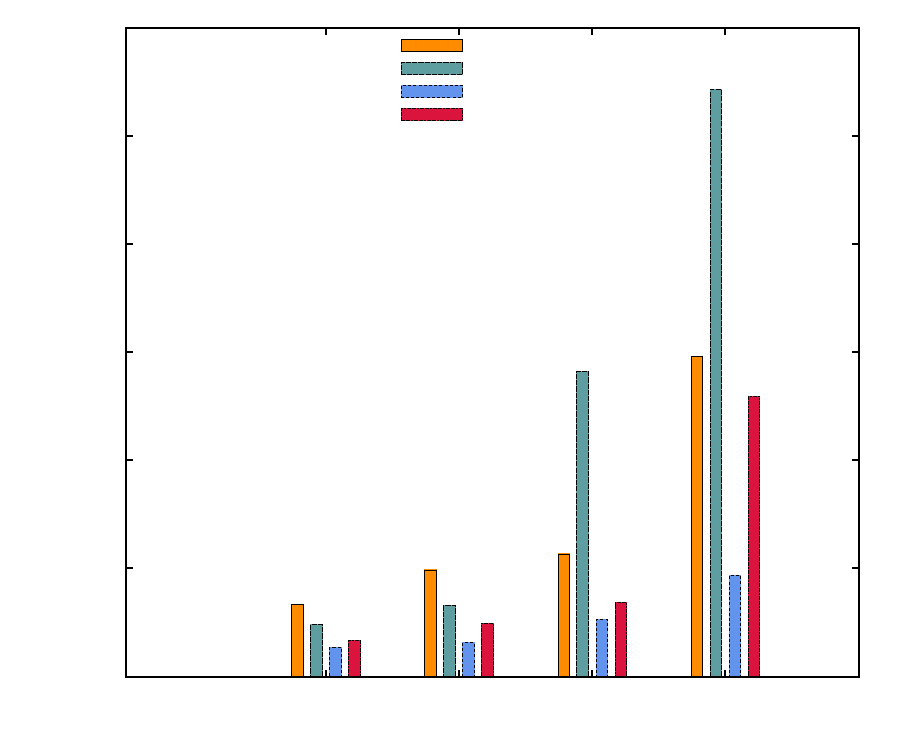
\includegraphics{chapter3/picFrequency/frequencyPlot}}%
    \gplfronttext
  \end{picture}%
\endgroup

	\caption[Mittlerer Abstand �ber Bildaufnahmefrequenz]{Gemittelter Abstand von der Fahrkurve �ber verschiedene Bildaufnahmefrequenzen mit vier verschiedenen Fahrkurven.}
	\label{fig:frequencyPlot}
\end{figure}

Die Ergebnisse sind in Abbildung \ref{fig:frequencyPlot} und \ref{fig:frequencyPlot_var} zu sehen. F�r alle vier Fahrkurven l�sst sich beobachten, dass sich bei sinkender Bildaufnahmefrequenz ein Anstieg des mittleren Abstandes zur tats�chlich gefahrenen Trajektorie ergibt. F�r die Fahrkurven \textbf{Ellipse} und \textbf{Loop~Anticlockwise} ist der Anstieg zwischen 500 und 2000\,$ms$ in etwa linear und macht ab 4000\,$ms$ einen Sprung. F�r die \textbf{Schlangenlinien} ist ein Sprung schon zwischen 1000 und 2000\,$ms$ zu sehen, mit einem weiteren zwischen 2000 und 4000\,$ms$. Bei \textbf{Loop~Clockwise} hingegen ist kein signifikanter Sprung zu erkennen.

Auch der mittlere lange Durchmesser der Ellipse w�chst bei sinkender Bildaufnahmefrequenz f�r alle Fahrkurven. Hier ist jedoch kein so signifikanter Sprung zu beobachten wie beim Abstand. Es l�sst sich nur ein unterschiedlich starker Anstieg im Durchmesser f�r die Fahrkurven ausmachen.
\begin{description}
\item[Loop~Clockwise] hat den geringsten Anstieg und hat von allen Fahrkurven, bei den untersuchten Bildaufnahmefrequenzen, den kleinsten mittleren Durchmesser der Unsicherheits-Ellipse.
\item[Loop~Anticlockwise] hat durchgehend den zweit kleinsten Durchmesser und einen Anstieg der nur knapp �ber \textbf{Loop~Clockwise} liegt.
\end{description}

\begin{figure}[h]
	\centering
	% GNUPLOT: LaTeX picture with Postscript
\begingroup
  \makeatletter
  \providecommand\color[2][]{%
    \GenericError{(gnuplot) \space\space\space\@spaces}{%
      Package color not loaded in conjunction with
      terminal option `colourtext'%
    }{See the gnuplot documentation for explanation.%
    }{Either use 'blacktext' in gnuplot or load the package
      color.sty in LaTeX.}%
    \renewcommand\color[2][]{}%
  }%
  \providecommand\includegraphics[2][]{%
    \GenericError{(gnuplot) \space\space\space\@spaces}{%
      Package graphicx or graphics not loaded%
    }{See the gnuplot documentation for explanation.%
    }{The gnuplot epslatex terminal needs graphicx.sty or graphics.sty.}%
    \renewcommand\includegraphics[2][]{}%
  }%
  \providecommand\rotatebox[2]{#2}%
  \@ifundefined{ifGPcolor}{%
    \newif\ifGPcolor
    \GPcolortrue
  }{}%
  \@ifundefined{ifGPblacktext}{%
    \newif\ifGPblacktext
    \GPblacktexttrue
  }{}%
  % define a \g@addto@macro without @ in the name:
  \let\gplgaddtomacro\g@addto@macro
  % define empty templates for all commands taking text:
  \gdef\gplbacktext{}%
  \gdef\gplfronttext{}%
  \makeatother
  \ifGPblacktext
    % no textcolor at all
    \def\colorrgb#1{}%
    \def\colorgray#1{}%
  \else
    % gray or color?
    \ifGPcolor
      \def\colorrgb#1{\color[rgb]{#1}}%
      \def\colorgray#1{\color[gray]{#1}}%
      \expandafter\def\csname LTw\endcsname{\color{white}}%
      \expandafter\def\csname LTb\endcsname{\color{black}}%
      \expandafter\def\csname LTa\endcsname{\color{black}}%
      \expandafter\def\csname LT0\endcsname{\color[rgb]{1,0,0}}%
      \expandafter\def\csname LT1\endcsname{\color[rgb]{0,1,0}}%
      \expandafter\def\csname LT2\endcsname{\color[rgb]{0,0,1}}%
      \expandafter\def\csname LT3\endcsname{\color[rgb]{1,0,1}}%
      \expandafter\def\csname LT4\endcsname{\color[rgb]{0,1,1}}%
      \expandafter\def\csname LT5\endcsname{\color[rgb]{1,1,0}}%
      \expandafter\def\csname LT6\endcsname{\color[rgb]{0,0,0}}%
      \expandafter\def\csname LT7\endcsname{\color[rgb]{1,0.3,0}}%
      \expandafter\def\csname LT8\endcsname{\color[rgb]{0.5,0.5,0.5}}%
    \else
      % gray
      \def\colorrgb#1{\color{black}}%
      \def\colorgray#1{\color[gray]{#1}}%
      \expandafter\def\csname LTw\endcsname{\color{white}}%
      \expandafter\def\csname LTb\endcsname{\color{black}}%
      \expandafter\def\csname LTa\endcsname{\color{black}}%
      \expandafter\def\csname LT0\endcsname{\color{black}}%
      \expandafter\def\csname LT1\endcsname{\color{black}}%
      \expandafter\def\csname LT2\endcsname{\color{black}}%
      \expandafter\def\csname LT3\endcsname{\color{black}}%
      \expandafter\def\csname LT4\endcsname{\color{black}}%
      \expandafter\def\csname LT5\endcsname{\color{black}}%
      \expandafter\def\csname LT6\endcsname{\color{black}}%
      \expandafter\def\csname LT7\endcsname{\color{black}}%
      \expandafter\def\csname LT8\endcsname{\color{black}}%
    \fi
  \fi
  \setlength{\unitlength}{0.0500bp}%
  \begin{picture}(8640.00,7200.00)%
    \gplgaddtomacro\gplbacktext{%
      \csname LTb\endcsname%
      \put(946,704){\makebox(0,0)[r]{\strut{} 0}}%
      \put(946,1483){\makebox(0,0)[r]{\strut{} 0.5}}%
      \put(946,2262){\makebox(0,0)[r]{\strut{} 1}}%
      \put(946,3041){\makebox(0,0)[r]{\strut{} 1.5}}%
      \put(946,3820){\makebox(0,0)[r]{\strut{} 2}}%
      \put(946,4598){\makebox(0,0)[r]{\strut{} 2.5}}%
      \put(946,5377){\makebox(0,0)[r]{\strut{} 3}}%
      \put(946,6156){\makebox(0,0)[r]{\strut{} 3.5}}%
      \put(946,6935){\makebox(0,0)[r]{\strut{} 4}}%
      \put(3032,484){\makebox(0,0){\strut{}500}}%
      \put(4335,484){\makebox(0,0){\strut{}1000}}%
      \put(5638,484){\makebox(0,0){\strut{}2000}}%
      \put(6940,484){\makebox(0,0){\strut{}4000}}%
      \put(176,3819){\rotatebox{-270}{\makebox(0,0){\strut{}Mittlerer langer Durchmesser der Ellipse in Metern}}}%
      \put(4660,154){\makebox(0,0){\strut{}Zeit zwischen zwei Bildern in Millisekunden}}%
    }%
    \gplgaddtomacro\gplfronttext{%
      \csname LTb\endcsname%
      \put(3586,6762){\makebox(0,0)[r]{\strut{}Ellipse}}%
      \csname LTb\endcsname%
      \put(3586,6542){\makebox(0,0)[r]{\strut{}Schlangenlinien}}%
      \csname LTb\endcsname%
      \put(3586,6322){\makebox(0,0)[r]{\strut{}Loop Clockwise}}%
      \csname LTb\endcsname%
      \put(3586,6102){\makebox(0,0)[r]{\strut{}Loop Anticlockwise}}%
    }%
    \gplbacktext
    \put(0,0){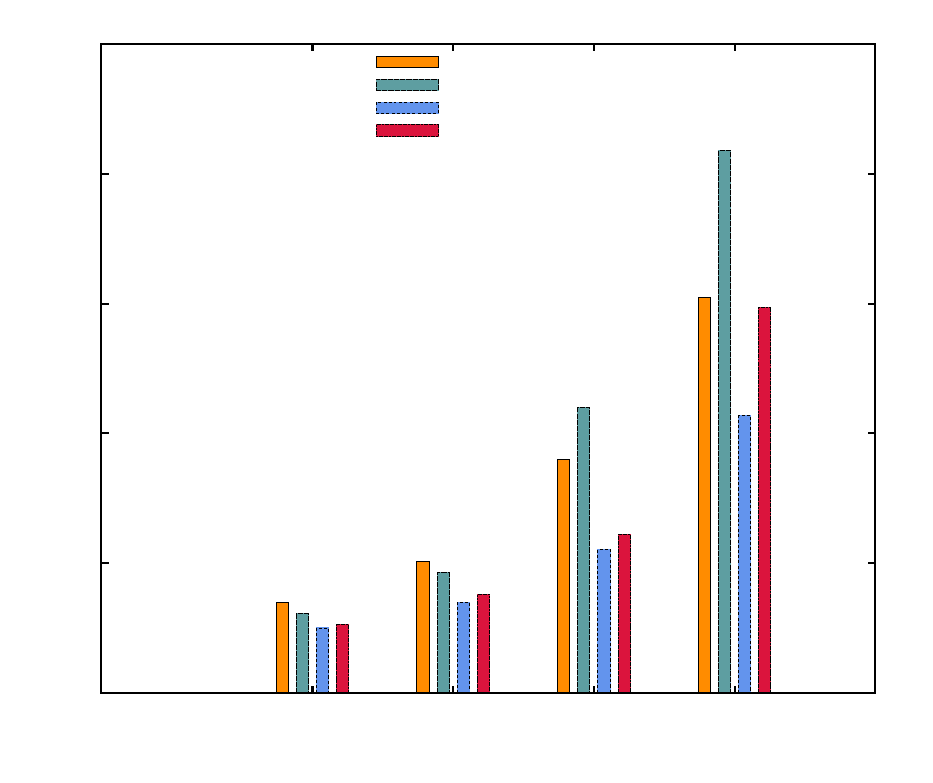
\includegraphics{chapter3/picFrequency/frequencyPlot_var}}%
    \gplfronttext
  \end{picture}%
\endgroup

	\caption{Gemittelter langer Durchmesser der Unsicherheits-Ellipse �ber verschiedene Bildaufnahmefrequenzen mit vier verschiedenen Fahrkurven.}
	\label{fig:frequencyPlot_var}
\end{figure}

\begin{description}
\item[Ellipse] liefert bei 500 und 1000\,$ms$ den gr��ten Durchmesser. Der Anstieg ist dabei aber nicht so stark wie bei den  \textbf{Schlangenlinien}.
\item[Schlangenlinien] sie zeigen die gr��te Zunahme beim Durchmesser. W�hrend sie zwischen 500 und 1000\,$ms$ an zweiter Stelle liegen, liefern sie zwischen 2000 und 4000\,$ms$ den gr��ten Durchmesser.
\end{description} 

\section{Versuche zum Einfluss von Menschen auf der B�hne}
\label{sec:VersucheCroud}
In diesem Versuch soll untersucht werden, wie stark Menschen auf der B�hne die Lokalisation mit dem hier vorgestellten Verfahren st�ren. Dabei geht es im wesentlichen darum, dass Menschen im Bild stehen und so die Bit-Muster ganz oder teilweise verdecken. Wie bei den Versuchen zur Bildaufnahmefrequenz wird auch hier der mittlere Abstand zur wahren Roboterposition verwendet. Als Fahrkurven werden ebenfalls die in Abschnitt \ref{sec:Fahrkurven} beschriebenen verwendet. Die Art der Durchf�hrung des Versuches wird nicht ver�ndert. Es wird jedoch anstatt des Zeitintervalls die Anzahl der Personen auf der B�hne ge�ndert (3,9,15,21). Das Zeitintervall f�r die Bildaufnahme wurde fest auf 1500\,$ms$ eingestellt.

\begin{wrapfigure}{o}{0.5\textwidth}
  	\center
    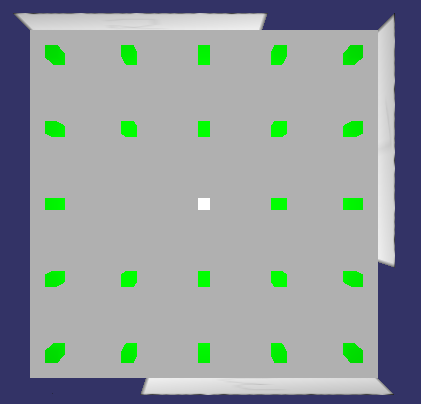
\includegraphics[width=0.45\textwidth]{chapter3/maxCrowd.png}
    \caption{M�gliche Positionen von Personen}
    \label{fig:maxCrowd}
\end{wrapfigure}
Es gibt 23 festgelegte Positionen f�r Personen auf der B�hne. Aus diesen wird bei jedem Simulationslauf zuf�llig die ben�tigte Anzahl ermittelt. Auf Abbildung~\ref{fig:maxCrowd} sind die m�glichen Positionen der Personen zu sehen. Wie in Abschnitt~\ref{sec:dieSzene} beschrieben sind die Personen 1800\,mm hoch und 400\,mm breit. Es ist davon auszugehen, dass je mehr Personen sich auf der B�hne befinden, es umso h�ufiger vorkommt, dass sie das Bit-Muster teilweise oder ganz verdecken. Bei einer hohen Personendichte sollte demnach der mittlere Abstand von der wahren Position gr��er werden. 
\begin{figure}[h]
	\centering
	% GNUPLOT: LaTeX picture with Postscript
\begingroup
  \makeatletter
  \providecommand\color[2][]{%
    \GenericError{(gnuplot) \space\space\space\@spaces}{%
      Package color not loaded in conjunction with
      terminal option `colourtext'%
    }{See the gnuplot documentation for explanation.%
    }{Either use 'blacktext' in gnuplot or load the package
      color.sty in LaTeX.}%
    \renewcommand\color[2][]{}%
  }%
  \providecommand\includegraphics[2][]{%
    \GenericError{(gnuplot) \space\space\space\@spaces}{%
      Package graphicx or graphics not loaded%
    }{See the gnuplot documentation for explanation.%
    }{The gnuplot epslatex terminal needs graphicx.sty or graphics.sty.}%
    \renewcommand\includegraphics[2][]{}%
  }%
  \providecommand\rotatebox[2]{#2}%
  \@ifundefined{ifGPcolor}{%
    \newif\ifGPcolor
    \GPcolortrue
  }{}%
  \@ifundefined{ifGPblacktext}{%
    \newif\ifGPblacktext
    \GPblacktexttrue
  }{}%
  % define a \g@addto@macro without @ in the name:
  \let\gplgaddtomacro\g@addto@macro
  % define empty templates for all commands taking text:
  \gdef\gplbacktext{}%
  \gdef\gplfronttext{}%
  \makeatother
  \ifGPblacktext
    % no textcolor at all
    \def\colorrgb#1{}%
    \def\colorgray#1{}%
  \else
    % gray or color?
    \ifGPcolor
      \def\colorrgb#1{\color[rgb]{#1}}%
      \def\colorgray#1{\color[gray]{#1}}%
      \expandafter\def\csname LTw\endcsname{\color{white}}%
      \expandafter\def\csname LTb\endcsname{\color{black}}%
      \expandafter\def\csname LTa\endcsname{\color{black}}%
      \expandafter\def\csname LT0\endcsname{\color[rgb]{1,0,0}}%
      \expandafter\def\csname LT1\endcsname{\color[rgb]{0,1,0}}%
      \expandafter\def\csname LT2\endcsname{\color[rgb]{0,0,1}}%
      \expandafter\def\csname LT3\endcsname{\color[rgb]{1,0,1}}%
      \expandafter\def\csname LT4\endcsname{\color[rgb]{0,1,1}}%
      \expandafter\def\csname LT5\endcsname{\color[rgb]{1,1,0}}%
      \expandafter\def\csname LT6\endcsname{\color[rgb]{0,0,0}}%
      \expandafter\def\csname LT7\endcsname{\color[rgb]{1,0.3,0}}%
      \expandafter\def\csname LT8\endcsname{\color[rgb]{0.5,0.5,0.5}}%
    \else
      % gray
      \def\colorrgb#1{\color{black}}%
      \def\colorgray#1{\color[gray]{#1}}%
      \expandafter\def\csname LTw\endcsname{\color{white}}%
      \expandafter\def\csname LTb\endcsname{\color{black}}%
      \expandafter\def\csname LTa\endcsname{\color{black}}%
      \expandafter\def\csname LT0\endcsname{\color{black}}%
      \expandafter\def\csname LT1\endcsname{\color{black}}%
      \expandafter\def\csname LT2\endcsname{\color{black}}%
      \expandafter\def\csname LT3\endcsname{\color{black}}%
      \expandafter\def\csname LT4\endcsname{\color{black}}%
      \expandafter\def\csname LT5\endcsname{\color{black}}%
      \expandafter\def\csname LT6\endcsname{\color{black}}%
      \expandafter\def\csname LT7\endcsname{\color{black}}%
      \expandafter\def\csname LT8\endcsname{\color{black}}%
    \fi
  \fi
  \setlength{\unitlength}{0.0500bp}%
  \begin{picture}(8640.00,7200.00)%
    \gplgaddtomacro\gplbacktext{%
      \csname LTb\endcsname%
      \put(1078,704){\makebox(0,0)[r]{\strut{} 0}}%
      \put(1078,1743){\makebox(0,0)[r]{\strut{} 0.05}}%
      \put(1078,2781){\makebox(0,0)[r]{\strut{} 0.1}}%
      \put(1078,3820){\makebox(0,0)[r]{\strut{} 0.15}}%
      \put(1078,4858){\makebox(0,0)[r]{\strut{} 0.2}}%
      \put(1078,5897){\makebox(0,0)[r]{\strut{} 0.25}}%
      \put(1078,6935){\makebox(0,0)[r]{\strut{} 0.3}}%
      \put(3128,484){\makebox(0,0){\strut{}3}}%
      \put(4407,484){\makebox(0,0){\strut{}9}}%
      \put(5686,484){\makebox(0,0){\strut{}15}}%
      \put(6964,484){\makebox(0,0){\strut{}21}}%
      \put(176,3819){\rotatebox{-270}{\makebox(0,0){\strut{}Mittlerer Abstand zum sollwert in Metern}}}%
      \put(4726,154){\makebox(0,0){\strut{}Anzahl an Personen auf der B�hne}}%
    }%
    \gplgaddtomacro\gplfronttext{%
      \csname LTb\endcsname%
      \put(3718,6762){\makebox(0,0)[r]{\strut{}Ellipse}}%
      \csname LTb\endcsname%
      \put(3718,6542){\makebox(0,0)[r]{\strut{}Schlangenlinien}}%
      \csname LTb\endcsname%
      \put(3718,6322){\makebox(0,0)[r]{\strut{}Loop Clockwise}}%
      \csname LTb\endcsname%
      \put(3718,6102){\makebox(0,0)[r]{\strut{}Loop Anticlockwise}}%
    }%
    \gplbacktext
    \put(0,0){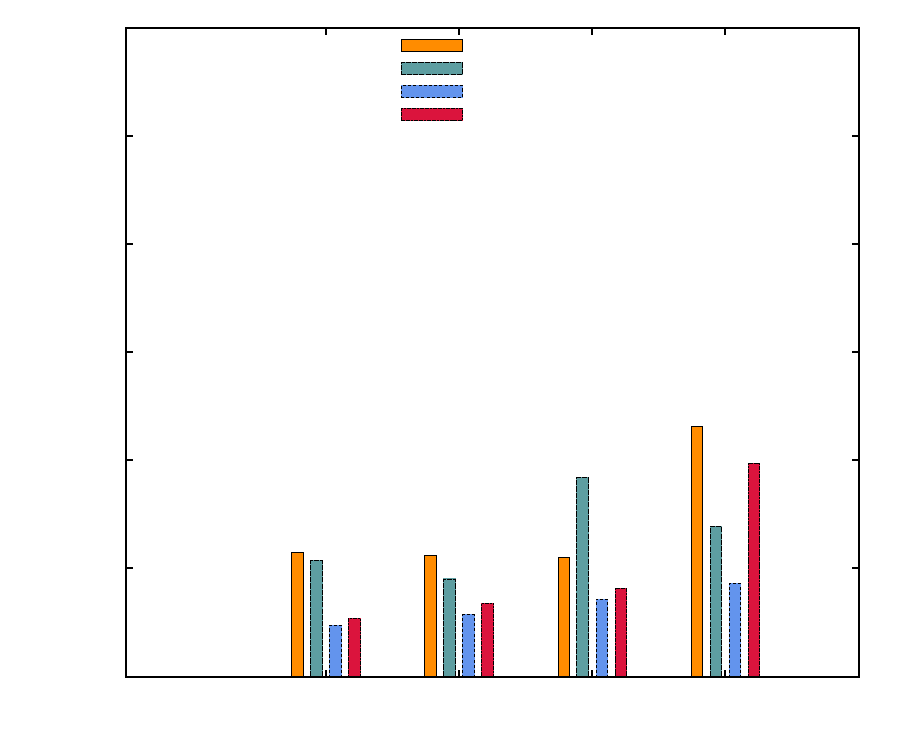
\includegraphics{chapter3/croudEffect/croudEffect}}%
    \gplfronttext
  \end{picture}%
\endgroup

	\caption{toller text}
	\label{fig:croudEffectPlot}
\end{figure}
  \chapter{Versuchsergebnisse}

  Vivamus ac hendrerit nisl. Morbi viverra sagittis urna, ac gravida diam posuere in. Nullam id enim nunc. Cras commodo eros ac mi iaculis ac aliquet eros molestie. Vestibulum semper, mauris a dapibus commodo, magna erat imperdiet ante, ac varius dolor ipsum et augue. Etiam non massa purus. Cras faucibus risus nec diam consectetur vestibulum. Donec luctus nunc eget diam commodo quis tempus augue mattis. Proin mattis mauris vehicula leo imperdiet tristique. Nullam a metus quam. Vivamus at turpis lorem, vel dapibus nisi.

  \chapter{Diskussion der Messergebnisse}

  Nulla ultrices accumsan turpis, at ultrices libero laoreet vitae. Nam ac ante in orci lobortis rutrum. Quisque metus diam, malesuada ac facilisis id, egestas eget dui. Donec id ante et ligula tincidunt congue. Ut eget neque eu sem elementum imperdiet. In euismod est id massa tristique eget vestibulum nisl lacinia. Nullam ullamcorper odio ut sem porta vulputate. Curabitur turpis turpis, tincidunt fermentum suscipit vel, vehicula quis nulla. Duis rhoncus sagittis condimentum. Ut molestie adipiscing mauris, vel imperdiet dui dignissim vel. Integer ac purus ante. Aenean euismod vulputate metus. Cras sit amet imperdiet ligula. Donec at diam diam. Donec posuere libero vel risus iaculis ullamcorper. Proin interdum pretium ante, eget rutrum felis elementum ut. Nam nisl nibh, sagittis in commodo vitae, venenatis non eros. Aenean pharetra vestibulum erat a tempor. Proin quam lacus, molestie a interdum id, consequat ac risus.
  \chapter{Fazit und Ausblick}
\label{chap:FazitundAusblick}
Es konnte gezeigt werden, dass das entwickelte Verfahren, in der erstellten Simulation, eine Lokalisation auf der B�hne erlaubt. Die durchgef�hrten Versuche zeigen den starken Einfluss der Trajektorie des Roboters auf der B�hne, insbesondere wenn nur wenige Bilder pro Minute ausgewertet werden k�nnen. Da Drehungen und Kurven die gr��te Quelle f�r Unsicherheiten sind haben sie den st�rksten Einfluss auf die gesch�tzte Position. Der Versuch zum Einfluss von Menschen auf der B�hne, welche die Bit-Muster verdecken k�nnen, lieferte keine aussagekr�ftigen Ergebnisse. Es l�sst sich nur festhalten, dass viele Personen auf der B�hne sich negativ auf die Lokalisation auswirken. Genauere Aussagen ben�tigen weitere Versuche, mit mehr Simulationsl�ufen. 
Der Ansatz des Verfahrens, nicht auf den Daten der Bilder zu arbeiten, konnte in der Simulation erfolgreich umgesetzt werden. 

R�ckblickend h�tten zus�tzlich Versuche durchgef�hrt werden k�nnen, um den Einfluss verschiedener Qualit�ten des Bit-Musters zu untersuchen. Ferner h�tten Testreihen zum Verhalten des Filters bei verschieden gew�hlten Unsicherheiten in der Simulation durchgef�hrt werden k�nnen.


Um das Verfahren weiter zu entwickeln, k�nnten weitere Versuche in der Simulation unternommen werden. Es k�nnte untersucht werden, wie gro� der Einfluss einer ungenauen Kamerakalibrierung auf die Lokalisation ist. Eine Erweiterung der Simulation w�re auch denkbar, indem die Lichtwand-Texturen mit einem Helligkeitsgradienten versehen werden. Ferne k�nnte die Lokalisation mit einem realen Roboter getestet werden. Dies w�rde ein Verfahren f�r die Kamerakalibrierung am Roboter voraussetzten. Es m�sste au�erdem beachtet werden, wie die Kamera am Roboter befestigt wird, da ein Drehen oder Verkippen eine erneute Kalibrierung erforderlich macht.
  \chapter{Fazit}
\label{chap:fazit}



  % gro�e r�mische Seitennummerierung
  \pagebreak
  \pagenumbering{Roman}
  \addtocontents{toc}{\protect\vspace{1cm}}

  % Anhang
  \begin{appendix}
    \chapter{Herleitung der Formel}

  \ac{LI} dolor sit amet, consectetur adipiscing elit. Etiam quam sapien, mattis non varius eu, rutrum eget nisl. Morbi venenatis molestie ante, sed aliquet lectus aliquet id. Pellentesque consectetur nisl a massa ornare congue. Curabitur pellentesque hendrerit dolor eget faucibus. Etiam non risus arcu, id fermentum elit. Quisque suscipit posuere semper. Vestibulum sit amet dolor nec risus malesuada interdum aliquam in turpis. Maecenas mollis, magna at porttitor fringilla, risus libero commodo justo, non tempus nibh massa lacinia sapien. Aenean sodales ullamcorper massa, eu ullamcorper ipsum tempus sed. In adipiscing congue scelerisque. Pellentesque molestie, quam vel dictum iaculis, metus nunc mollis mi, nec venenatis tellus turpis eu arcu. Praesent at ultricies nibh. Proin neque libero, tincidunt dignissim ornare in, sagittis in ligula. Nunc sagittis sodales massa, a tempus felis vehicula id. Cum sociis natoque penatibus et magnis dis parturient montes, nascetur ridiculus mus. Nulla adipiscing vestibulum eros, ut imperdiet augue scelerisque id. Vestibulum ante ipsum primis in faucibus orci luctus et ultrices posuere cubilia Curae; Suspendisse aliquam pulvinar lectus id dictum. Etiam dictum sollicitudin elit sed scelerisque. Nullam sodales semper interdum.

    \chapter{�ber das Problem X}

  Sed turpis erat, tincidunt eu sollicitudin eu, tempus quis lectus. Nullam orci leo, tempus vitae dictum eu, bibendum at ante. In placerat, mi eu consequat suscipit, turpis arcu dictum tellus, nec scelerisque turpis eros a enim. Mauris quis leo lacus. Vestibulum condimentum porttitor malesuada. Pellentesque nec dictum nisl. Donec eleifend libero sit amet urna dignissim in faucibus lorem ultricies. Vestibulum interdum egestas metus vel porta. In vehicula leo at nibh dignissim malesuada. Etiam non nunc ligula. Vivamus vitae nibh dolor, eget faucibus tortor. Suspendisse ac quam enim. 


    % Abk�rzungsverzeichnis
    \chapter{Abk�rzungsverzeichnis}

  \begin{acronym}[YTM]
    \acro{CDT}{C/C++ Development Tools}
    \acro{OCG}{Open Scene Graph}
    \acro{BBM}{Beobachter der Bediener von Maschinen}
  \end{acronym}


    % Quellenverzeichnis
    \bibliography{quellen}
  \end{appendix}

% Dokument beenden
\end{document}
